\documentclass[%
    fontsize=11pt, %font size
    paper=a4, %paper format
    headsepline, %separating line for header
    chapterprefix, % produce "Chapter ..."
    numbers=noenddot, % no full-stop after last number
    listof=totoc, %Entry in table of contents for list of figures/tables
    bibliography=totoc, %Entry in table of contents for bibliography
    BCOR=5mm %Binding correction, ensures sufficient space for binding
]%
{scrbook}%

\usepackage{scrbase} %Hilfsfunktionen
\usepackage{ellipsis, fixltx2e, mparhack, ragged2e} %bugfixing
\usepackage[l2tabu, orthodox]{nag} %avoid typical LaTeX errors

\usepackage[english]{babel}
\usepackage[T1]{fontenc} % Fonts
\usepackage{lmodern}
\usepackage[utf8]{inputenc} % Unicode input
\usepackage[final]{microtype} %microtypography

\usepackage{graphicx}
\usepackage{subcaption}
\usepackage{tabularx}
\usepackage{booktabs}
\usepackage{xspace}
\usepackage{acro}
\usepackage{enumitem}
\usepackage[autostyle=true]{csquotes}

\usepackage[marginclue,langtrack]{fixme}

\usepackage{amsmath}
\usepackage{amssymb}
\usepackage{amsthm}
\usepackage{bm}
\usepackage{amsfonts}
\usepackage{isomath}	% for \mathbfit
\usepackage{esint}		% suface integrals
\usepackage{mathtools}	% for definition symbol \coloneqq
\usepackage{upgreek}
\usepackage{siunitx}

\usepackage{tikz}
\usetikzlibrary{calc}
\usetikzlibrary{decorations.markings}
\usetikzlibrary{patterns}

\usepackage{pgfplots}
\pgfplotsset{compat=newest}
\pgfplotsset{table/search path = {./../../numerical_results/}}
\usepgfplotslibrary{external} 
\tikzexternalize[prefix=./external_figures/]

% Bibliography
\usepackage[%
    style=ieee,
    backend=biber,
    url=true,
    isbn=false,
    doi=false,
    ]%
{biblatex}
\addbibresource{./../references.bib}

\usepackage[%
    pdfauthor={Simon Sturm},
    hidelinks,
    % colorlinks=true,
    linkcolor=blue,
    filecolor=magenta,      
    urlcolor=cyan,
    pdfpagemode=FullScreen,
    breaklinks=true, %% allow links to break across lines
    hyperfootnotes=false% incompatible with package footmisc
]%
{hyperref}%

\usepackage[english,capitalise]{cleveref} % After loading hyperref!

%%%%%%%%%%%%%%%%%%%%%%%%%%%%%%%%%%%%%%%%%%%%%%%%%%%%%%%%%%%%%%%%%%%%%%%%%%%%%%%%
% Abbreviations
%%%%%%%%%%%%%%%%%%%%%%%%%%%%%%%%%%%%%%%%%%%%%%%%%%%%%%%%%%%%%%%%%%%%%%%%%%%%%%%%
\newcommand{\ie}{i.\,e.\xspace}%
\newcommand{\eg}{e.\,g.\xspace}%
\newcommand{\wrt}{w.\,r.\,t.\xspace}%

%%%%%%%%%%%%%%%%%%%%%%%%%%%%%%%%%%%%%%%%%%%%%%%%%%%%%%%%%%%%%%%%%%%%%%%%%%%%%%%%
% Acronyms
%%%%%%%%%%%%%%%%%%%%%%%%%%%%%%%%%%%%%%%%%%%%%%%%%%%%%%%%%%%%%%%%%%%%%%%%%%%%%%%%

\DeclareAcronym{CE}{
    short = CE,
    long = computational electromagnetics
    }
\DeclareAcronym{ODE}{
    short = ODE,
    long = ordinary differential equation,
    short-plural = s,
    long-plural = s
    }
\DeclareAcronym{LSE}{
    short = LSE,
    long = linear system of equations,
    }
\DeclareAcronym{PDE}{
    short = PDE,
    long = partial differential equation,
    short-plural = s,
    long-plural = s
    }
\DeclareAcronym{PEC}{
    short = PEC,
    long = perfect electric conductor
    }
\DeclareAcronym{PMC}{
    short = PMC,
    long = perfect magnetic conductor
    }
\DeclareAcronym{FMM}{
    short = FMM,
    long = fast multipole method
    }
\DeclareAcronym{MLFMA}{
    short = MLFMA,
    long = multilevel fast multipole algorithm
    }
\DeclareAcronym{DCIM}{
    short = DCIM,
    long = discrete complex image method
    }
\DeclareAcronym{GPOF}{
    short = GPOF,
    long = generalized penicl-of-function method
    }
\DeclareAcronym{CSB}{
    short = CSB,
    long = complex-source beam,
    short-plural = s,
    long-plural = s
    }
\DeclareAcronym{EIT}{
    short = EIT,
    long = exact image theory
    }
\DeclareAcronym{MoM}{
    short = MoM,
    long = method of moments
    }
\DeclareAcronym{FDM}{
    short = FDM,
    long = finite difference method,
    short-plural = s,
    long-plural = s,
    }
\DeclareAcronym{FEM}{
    short = FEM,
    long = finite element method,
    }
\DeclareAcronym{HD}{
    short = HD,
    long = Hertzian dipole,
    short-plural = s,
    long-plural = s,
    }
\DeclareAcronym{VED}{
    short = VED,
    long = vertical electric dipole,
    short-plural = s,
    long-plural = s,
    }
\DeclareAcronym{HED}{
    short = HED,
    long = horizontal electric dipole,
    short-plural = s,
    long-plural = s,
    }
\DeclareAcronym{VMD}{
    short = VMD,
    long = vertical magnetic dipole,
    short-plural = s,
    long-plural = s,
    }
\DeclareAcronym{HMD}{
    short = HMD,
    long = horizontal magnetic dipole,
    short-plural = s,
    long-plural = s,
    }
\DeclareAcronym{TL}{
    short = TL,
    long = transmission line,
    short-plural = s,
    long-plural = s,
    }
\DeclareAcronym{TLGF}{
    short = TLGF,
    long = transmission line Green's function,
    short-plural = s,
    long-plural = s,
    }
\DeclareAcronym{TM}{
    short = TM,
    long = transversally magnetic
    }
\DeclareAcronym{TE}{
    short = TE,
    long = transversally electric
    }
\DeclareAcronym{CG}{
    short = CG,
    long = conjugate gradient method
    }
\DeclareAcronym{GMRES}{
    short = GMRES,
    long = generalized minimal residual algorithm
    }
\DeclareAcronym{RWG}{
    short = RWG,
    long = Rao Wilton Glisson
    }
\DeclareAcronym{SIP}{
    short = SIP,
    long = Sommerfeld integration path
    }
\DeclareAcronym{EIP}{
    short = EIP,
    long = extended integration path
    }
\DeclareAcronym{PE}{
    short = PE,
    long = partition-extrapolation
    }

%%%%%%%%%%%%%%%%%%%%%%%%%%%%%%%%%%%%%%%%%%%%%%%%%%%%%%%%%%%%%%%%%%%%%%%%%%%%%%%%
% Theorem environments
%%%%%%%%%%%%%%%%%%%%%%%%%%%%%%%%%%%%%%%%%%%%%%%%%%%%%%%%%%%%%%%%%%%%%%%%%%%%%%%%

\theoremstyle{theorem}
\newtheorem{theorem}{Theorem}[section]

\theoremstyle{corollary}
\newtheorem{corollary}{Corollary}[theorem]

\theoremstyle{lemma}
\newtheorem{lemma}[theorem]{Lemma}

\theoremstyle{definition}
\newtheorem{definition}{Definition}[section]
\newtheorem{remark}{Remark}[theorem]

%%%%%%%%%%%%%%%%%%%%%%%%%%%%%%%%%%%%%%%%%%%%%%%%%%%%%%%%%%%%%%%%%%%%%%%%%%%%%%%%
% Own mathematical commands
%%%%%%%%%%%%%%%%%%%%%%%%%%%%%%%%%%%%%%%%%%%%%%%%%%%%%%%%%%%%%%%%%%%%%%%%%%%%%%%%

% Physical and geometrical vectors
\newcommand{\pvec}[1]{\mathbfit{#1}}     	% general "physical" vector and vector in frequency domain
\newcommand{\tdvec}[1]{\bm{\mathfrak{#1}}}	% time domain
\newcommand{\uv}[1]{\hat{\pvec{#1}}} 		% unit vector
\newcommand{\dyad}[1]{\overline{\pvec{#1}}}
\renewcommand{\vec}[1]{\mathsfbfit{#1}} 	% n-dimensional vector
\newcommand{\mat}[1]{\mathsfbfit{#1}} 		% <n x n> matrix

% Operators
\newcommand{\op}[1]{\mathcal{#1}} 			% operator that takes a scalar-valued function
\newcommand{\vecop}[1]{\bm{\mathcal{#1}}} 	% operator that takes a vector-valued function
\DeclareMathOperator{\laplace}{\Delta}		% scalar Laplacian operator
\DeclareMathOperator{\laplaceTrans}{\laplace_\mathrm{t}}	% transversal Laplacian operator
\DeclareMathOperator{\gradient}{\nabla}		% gradient operator
\DeclareMathOperator{\divergence}{\nabla\cdot}		% divergence operator
\DeclareMathOperator{\curl}{\nabla\times}			% curl operator
\newcommand{\abs}[1]{\left\vert#1\right\vert}	% absolute value
\newcommand{\norm}[1]{\left\Vert #1 \right\Vert}
\newcommand{\euclideanNorm}[1]{\norm{#1}_2} % Euclidean norm
\newcommand{\complexLength}[1]{\norm{#1}_\mathrm{c}} % Euclidean norm
\newcommand{\pd}[2][]{\frac{\partial#1}{\partial#2}} 	% partial derivative (function as an optional argument)
\newcommand{\nd}[2][]{\frac{\dd#1}{\dd#2}} 	% normal derivative (function as an optional argument)
\newcommand{\pdsec}[1]{\frac{\partial^2}{\partial {#1}^2}}	% 2nd partial derivative
\newcommand{\pdsecmixed}[2]{\frac{\partial^2}{\partial {#1} \partial {#2}}}	% 2nd mixed partial derivative
\newcommand{\landau}[1]{\mathcal{O} \left( #1 \right)}
\newcommand{\cmplxlength}[1]{\abs{#1}_\mathrm{c}}

% Integral transforms
\newcommand{\fourierTransformTemporal}{\mathcal{F}_{\mathrm{t}}}
\newcommand{\fourierTransformTemporalInverse}{\mathcal{F}_{\mathrm{t}}^{-1}}
\newcommand{\fourierTransformSpatial}{\mathcal{F}_{\mathrm{s}}}
\newcommand{\fourierTransformSpatialInverse}{\mathcal{F}_{\mathrm{s}}^{-1}}
\newcommand{\hankelTransform}[1]{\mathcal{H}_{#1}}
\newcommand{\hankelTransformInverse}[1]{\mathcal{H}^{-1}_{#1}}
\newcommand{\sommerfeldIntegral}[1]{\mathcal{S}_{#1}}

% Misc
\newcommand{\e}{\mathrm{e}}					% Euler's number
\renewcommand{\exp}[1]{\e^{#1}\,}			% exponential function
\renewcommand{\pi}{\uppi}
\newcommand{\dd}{\mathrm{d}}  				% the differential symbol is actually an operator
\DeclareMathOperator{\const}{const.}

% Complex numbers
\newcommand{\im}{\mathrm{j}}
%\renewcommand{\Re}{\mathrm{Re}\;}
%\renewcommand{\Im}{\mathrm{Im}\;}
\newcommand{\real}[1]{\Re\mathrm{e}\left(#1\right)}
\newcommand{\imag}[1]{\Im\mathrm{m}\left(#1\right)}

% Blackboard font: for special sets of numbers
\newcommand{\C}{\mathbb{C}}	% complex numbers
\newcommand{\R}{\mathbb{R}}	% real numbers
\newcommand{\N}{\mathbb{N}}	% natural numbers
\newcommand{\Z}{\mathbb{Z}}	% integers
\newcommand{\F}{\mathbb{F}}	% a general field

% Special functions
\DeclareMathOperator{\diracDelta}{\updelta}
\newcommand{\besselj}[1]{\operatorname{J}_{#1}}
\newcommand{\sphbesselj}[1]{\operatorname{j}_{#1}}
\newcommand{\besselh}[2]{\operatorname{H}_{#2}^{\left( #1 \right)}}
\newcommand{\sphbesselh}[2]{\operatorname{h}_{#2}^{\left( #1 \right)}}
\newcommand{\legendrepl}[1]{\operatorname{P}_{#1}}

% Custom commands for this thesis
\newcommand{\robs}{\pvec{r}}
\newcommand{\rsrc}{\pvec{r}^\prime}
\newcommand{\rdiff}{\robs-\rsrc}
\newcommand{\rdiffabs}{\abs{\rdiff}}
\newcommand{\ewaldintegral}{\oiint\limits_{S^2} \dd^2 \uv{k} \, }
\newcommand{\te}{\mathrm{TE}}
\newcommand{\tm}{\mathrm{TM}}
\newcommand{\tx}{\mathrm{TX}}
\newcommand{\isrc}{\mathrm{i}}
\newcommand{\vsrc}{\mathrm{v}}

\newcommand{\epsr}[1][]{\varepsilon_{\mathrm{r}#1}} 	% relative permittivity (layer index as an optional argument)
\newcommand{\mur}[1][]{\mu_{\mathrm{r}#1}} 	% relative permeability (layer index as an optional argument)

% FMM definitions
\newcommand{\fmmDiffGroupCenters}{\pvec{t}_{m,m^\prime}}
\newcommand{\fmmGroupCenter}[1]{\pvec{c}_{#1}}
\newcommand{\fmmSrcGroupCenter}{\pvec{c}_{m^\prime}}
\newcommand{\fmmObsGroupCenter}{\pvec{c}_{m}}
\newcommand{\fmmMultiIndex}{\vec{m}}



\fxsetup{draft}
%\fxsetup{final}

\begin{document}

\tableofcontents

\chapter{Introduction}
\label{ch:introduction}

\section{Background}

The references at the end of this document thematically are all part of an area
which could be enveloped as \emph{electromagnetic theory and practical field
computation.}
The overall contribution of some of these publications to the area might be
marginal.
Some might be beneficial in solving certain problems at hand.
Some might be seminal \cite{Sommerfeld1909}.
One --- without any doubt --- \emph{is} epochal
\cite{maxwell1865}.

Although it is very unlikely these days that anybody will actually consider the
original set of twenty equations published by the great man himself in 1865
\cite{maxwell1865} when using the term \enquote{Maxwell's equations} ---
it was to the Scottish mathematician and physicist to first bring together the
pieces of insight gained by other major names during the early 19th century and
to supplement the fragments to a theory of utmost elegance and predictive power.

In defiance of the elegance and relative simplicity of electromagnetic theory
the field problem can only be solved analytically for a finite set of the most
simple and highly symmetrical problems.
Even some of those problems have forced past generations to apply and in some
cases even develop sophisticated mathematical formalisms \cite{Felsen1994}.
In modern times, however, the advances in powerful computers enables the use of  
numerical methods to solve the field problem for more real-world scenarios in
principle up to the accuracy of machine precision.
Some of these methods were even known for a long time, but had to await
practical applicability until major computational power was available.

A particularly pleasant circumstance, however, is that many of the ancestral
analytical efforts have by no means become obsolete --- they rather can be used
beneficially in powerful numerical methods.
The example which is subject to this thesis is the use of fundamental solutions
\textemdash so-called Green's functions \textemdash within the framework
provided by the \ac{MoM} \cite{Harrington1993}.

The particular problem motivating this thesis is to find a combination of
different numerical methods which all employ analytical results in a very
distinguished way. Namely, the Green's function of the so-called half-space
problem shall be used in conjunction with the \ac{FMM} in order to accelerate
the numerical solution of field problems formulated in terms of integral
equations.

\section{Sommerfeld Half-Space Problem and Multilayered Media}

An outstanding both for the prosperous use of analytical techniques and for the
gainful use of so obtained results in numerical techniques is the Green's 
function of the half-space problem and closely related multilayered media.

The first goes back to the seminal publications of Arnold Sommerfeld in the
early days of radio and antennas \cite{Sommerfeld1909}.
He first considered a vertically oriented \ac{HD}, residing at the interface
formed by semi-unbounded free-space and the surface of the earth.
The latter is assumed to be flat and to possess lossy dielectric material
properties.
With his work Sommerfeld mathematically verified the assumed existence of
a special kind of surface wave \cite{Zenneck1907} and examined how the separate
constituents of the total wave field correspond to purely mathematical
attributes of the underlying formalism.
This, in conjunction to the first-place development of this very formalism is
the cause why Sommerfeld's 1909 paper is rewarded as pioneering down to the
present day \cite{Michalski2015, Michalski2016b, Mosig2021}.
Sommerfeld later elaborated more on the topic
\cite{Sommerfeld1926,Sommerfeld1964}, \eg, generalizing it to the \ac{HED}
case and to a situation where the dipole is located above the interface
At least in the 1926 paper \cite{Sommerfeld1926} a small but controversially
discussed sign error from the original paper \cite{Wait1998} was fixed.

Sommerfeld's formalism was later generalized to arbitrary solution domains
compound by several plane layers \cite{Felsen1994, Michalski1990},
possibly even ones with anisotropic material parameters and \ac{PEC}, \ac{PMC}
as well as impedance boundary conditions \cite{Hsu1993, Michalski2005}.

\fxnote{Sommerfeld originally \cite{Sommerfeld1909} solved for the vector
potential of the \ac{VED} (\enquote{Hertz potential})}

\section{Numerical Evaluation of Sommerfeld Integrals}

General (no PDF):
\cite{mosig1982}

Path deformation
\cite{Michalski1985a}

Tails, \ac{PE}
\cite{Michalski1998}
\cite{Mosig2012}
\cite{mosig2013}
\cite{Michalski2016a}
\cite{Golubovic2012}

Head DE rules
\cite{golubovicniciforovic2011}

Head detour semi-elliptical
\cite{GayBalmaz1997}

Head detour roof-top
\cite{Michalski2015a}

MPM
\cite{MengtaoYuan2006a}

\ac{SIP}, \ac{EIP} only for $\rho$ up to a few hundred wavelenghts \cite[p.~14]{Michalski2016b}
Reason: not the tail \ac{PE} but rapid oscillations in head

\section{Closed Form Approximations}

\section{Integral Equation Techniques and the Method of Moments}

\cite{Harrington1993}

Integral equations arising from boundary value problems in \ac{CE} can be
discretized by subdomain basis functions, \eg, the popular \ac{RWG} functions
\cite{Rao1982}.

Direct solver: $N^3$
Iterative solver: $N^2$

\section{Fast Multipole Method}

\subsection{Motivation}

Due to the global nature of the involved Green's functions the discretization
of \ac{MoM}-based discretization of integral equations lead to a dense \ac{LSE}.
These systems are most commonly solved using iterative solvers in which the
system matrix is applied to a several, recursively generated, excitation
vectors until the solution has converged to the desired accuracy.
Popular examples for iterative solvers are multiple versions of the \ac{CG}
or the \ac{GMRES} \cite{Strang2010}.

If now, in a Galerkin-type \ac{MoM} scheme, $N$ denotes the number of expansion
and testing functions, each single matrix-vector multiplication exhibits a
complexity of $\landau{N^2}$ in terms of operations as well as in terms of
memory. Since this becomes prohibitive for large $N$ as occurring in
field computations of many real-world problems, an extensive set of fast
algorithms has been developed which all aim to accelerate matrix-vector
multiplication \cite[chapter 11]{Jin2015}.

One such fast method is the \ac{FMM} and, as an extension of the latter, the
\ac{MLFMA}. In principle these algorithms are capable to reduce the complexity
to $\landau{N^{3/2}}$ and even $\landau{N \log N}$, respectively.
As opposed to some other fast algorithms, the \ac{FMM} is problem
specific. 
Nevertheless, 2D \cite{Rokhlin1990} and 3D \cite{Rokhlin1993, Coifman1993}
versions of the \ac{FMM} have been developed for the major equation in
full-wave \ac{CE}, the Helmholtz equation.
Today the use of the \ac{MLFMA} is state of the art in the treatment of
large-scale problems with integral equation techniques\footnote{Interestingly,
in the early days of the \ac{FMM} even its creators assumed that it would not be
beneficial to improve the method to a $\landau{N \log N}$ algorithm by
applying the scheme recursively several times. The reason is they assumed
\enquote{problems of practicable size} to be not larger than
$N \le \num{1000000}$ \cite{Rokhlin1993}.}
The involved algorithms, data structures and the choice of important
parameters have been extensively studied and  are well-documented
\cite{Chew2001}.

\subsection{Principle}

The starting point in the development of the \ac{FMM} is the Green's function
of free space.
The core idea, interpreted in terms of electrodynamics, is as follows.
In order to solve the field problem for a general distribution of $N$ sources
of radiation --- we may assume $N$ \acp{HD} radiating into free space ---
one has to evaluate the corresponding Green's function $N^2$ times.
This is due to the interaction of every \ac{HD} with every other one.
If now the \acp{HD} are not distributed equally in space but somewhat are
\emph{clustered} the idea of a multipole expansion 
\cite[9.7]{Jackson2013} \cite[7.10]{vanBladel2007} comes into place.
The claim is that in a cluster of \acp{HD} each individual \ac{HD} will not
\enquote{see} every single \ac{HD} in a cluster of \acp{HD} which is far away.
Instead, it will be sufficient to consider only bigger entities, namely the
whole clusters, in terms of far interaction while the near interactions
between individual \acp{HD} need to be considered only within the clusters.
Concisely formulated the \ac{FMM} consists of the following three steps. 
\begin{enumerate}
	\item The effects of all individual \acp{HD} within a cluster of sources
	are \emph{aggregated} to a common center within the respective group. 
	\item The aggregated effect is \emph{translated} to the common reference
	point of a far-away group of, likewise clustered, observing \acp{HD}.
	\item Within the group of observing \acp{HD} the translated quantity is
	redistributed or \emph{disaggregated} to all individual receiving \acp{HD}.
\end{enumerate}

These steps somewhat correspond to a factorization of the Green's function
into a product of three factors.

The same principle sketched here for point-like sources can easily be extended
to arbitrary basis and testing functions within the \ac{MoM} by invoking
the linearity of Maxwell's equations and the superposition principle.

Since the described approach only works for far-interactions of properly
clustered groups of \acp{HD} or --- more general --- subdomain basis functions 
of local support, all the possible near-interactions need to be treated
separately.
This can be done applying the conventional \ac{MoM} approach to compute all
nearby interactions.
The effect here is, that the \ac{FMM} removes all entries in the system matrix
which would not be centered around its diagonal within the standard \ac{MoM}.
The result is a sparse and banded matrix, similar to those resulting from
techniques based on differential equations, such as the \ac{FEM} or certain
forms of \acp{FDM}.
This resulting sparse matrix is then much easier to treat than the corresponding
full \ac{MoM} matrix. At the same time the obtained algorithm benefits from the
reduced number of unknowns as compared to differential equation techniques.

\subsection{Extension to Source Points in Complex Space}

The use of complex vectors \cite[Chapter 1]{Lindell2000} is omnipresent within
the study of time-harmonic electromagnetic fields.
However, vectors in $\C^3$ are usually \emph{electromagnetic} quantities like
vector potentials and the fields themselves.
In contrast, (arbitrary) complex spatial coordinates are rather uncommon so
far\footnote{Counterexamples are found, \eg, within the context of Lorentz
transforms between moving frames of reference, where angles of rotation may be
imaginary \cite[Chapter~11]{Jackson2013}.}.
An example use case in which the concept of complex space plays a prominent role
is given in a paper by \textcite{Hansen2009}, where a new perspective on the
classical Huygens principle based on complex source locations is presented. 

It is well-known that if the Green's function of the scalar Helmholtz equation
for the free-space case describes a spherical wave for the usual case where
the distance between source and observation point is a real number.
This pattern changes if this distance is complex.
In this case the magnitude of the wave field becomes dependent on direction.
This kind of wave field is commonly called Gaussian beam or \ac{CSB}.
Albeit the concept of \emph{complex space} is somewhat abstract
\cite[Chapter~1]{Lindell2000}, an intuitive and commonly employed definition of
\emph{complex length} is, that such a quantity should have a positive real part
\cite{Hansen2009, Hansen2013}.

Concerning the combination of the \ac{FMM} with sources situated in complex
space, it appears obvious that this kind of application was not what the
creators originally had in mind.
The popular review paper by \textcite{Coifman1993}, for example, does not make
any indications towards this direction.
Interestingly enough, in the mathematically rigorous treatment of the 3D
\ac{FMM} for the Helmholtz equation \cite{Rokhlin1993}, the essential
Theorem~2.2 is formulated in terms of complex spatial coordinates and even
complex angles.
However, these assumptions are dropped as early in the following as in
Theorem~2.3, whose requirements assume real spatial quantities and leave only
the wavenumber in the complex domain.
The same assumptions underlie the mathematically oriented publication Concerning
the 2D \ac{FMM} \cite{Rokhlin1990}.

From these observations it appears obvious, that the \ac{FMM} development
made no efforts towards an applicability to sources (or observation points)
situated in whatever form of complex space.
Actually in most cases of application even the wavenumber is simply the one of
free space and is therefore real quantity.

Nevertheless, a combination of the concept of \acp{CSB} with the \ac{FMM} can
provide benefits.
Employing some earlier results \cite{Hansen2009}, it was shown by
\textcite{Hansen2013}, that the introduction of a well-defined
\emph{imaginary shift} applied to the basis functions in a \ac{FMM} setup
results in a modified \ac{FMM} translation operator which shows a significantly
directive pattern.
This so-called Gaussian translation operator allows to neglect some plane wave
directions involved in the expansion throughout the translation step
and therefore renders the resulting algorithm computationally more effective
than a \ac{FMM} using the standard translation operator.

It should be noted that the requirements in the derivation of the Gaussian
translation operator and also the corresponding proof 
\cite[Appendix]{Hansen2013} do not assume general source points located in
complex space defined in a sense that all three spatial coordinates might
be arbitrary complex numbers.
The imaginary part of the source position vector is instead selected by a given
intention regarding the sharpness of the resulting \ac{CSB}.
Consequently, the parameter controlling the imaginary shift of source points
is labeled \emph{beam parameter} by the author.

\fxnote{\cite{Borries2014}}

In the course of the literature research for this thesis no thoroughly and 
mathematically rigorous treatment was found concerning the combination
of the \ac{FMM} principle with actual complex source points located at
\emph{arbitrary} \enquote{positions} in a complex version of Euclidean space.

However, there are records of some attempts to do so using a standard \ac{FMM}
implementation and without the aim of extending the underlying theorems and
proofs \cite{Rokhlin1993}.
A rather heuristic discussion of this topic is given in a paper by
\textcite{Geng2001}.
It is empirically shown that the use of complex source points drastically
deteriorates the convergence of the central addition theorem on which the
\ac{FMM} is based.
The number of terms in the corresponding series expansion is closely
related to the number of quadrature points required to numerically integrate
the plane-wave expansion --- the second main identity within the
\ac{FMM}.
For this reason the authors did not pursue the approach of using complex images
further and instead directed their attention to approximate forms of the
Green's function using a single real image source for all far interaction
computed using the \ac{FMM} \cite{Geng1999, Geng2000}.

\subsection{Adaption to Half-Space Green's Functions}

\cite{Geng2000}
\cite{Liu2002}
\cite{Eibert2018}
\cite{Eibert2018a}
\cite{Eibert2019}
\cite[Chapter~8.13.2]{parini2020}

\part{Theoretical Considerations}
\label{part:theory}






\chapter{Mathematical Preliminaries}
\label{ch:math_preliminaries}

The aim of this chapter is, in first place, to provide a unified
treatment of major ideas and theorems which form the foundation of the study
of electromagnetic ware propagation in half-space environments and
multilayered media.
Secondly, important consequences for the topic at hand---namely the computation
of highly accurate reference results and the aspired combination of the \ac{FMM}
with the Sommerfeld problem's solution domain---are pointed out.




\section{Notation}

Let the following notes regarding notation prepended this chapter.
\begin{itemize}
	\item Real and complex numbers are marked in the
	respective context if necessary.
	For an arbitrary complex number $z \in C$ the complex 
	conjugate is denoted by $\complexConjugate{z}$ and the absolute value of
	$z$ is written as $\abs{z} = \sqrt{z \complexConjugate{z}}$.
	The symbol $\im \coloneqq \sqrt{-1}$ is used as imaginary unit.
	\item Vectors in $\R^3$ with a physical meaning are
	denoted in bold and italic serif font, \eg, the position vector $\pvec{r}$.
	Source points are marked by a prime.
	Unit vectors are marked by a hat, \eg, $\uv{u}$.
	\item Entities with reference to linear algebra, \ie,
	matrices and vectors are denoted in bold, italic and sans-serif font.
	Matrices, \eg, $\mat{A}$, are distinguished from column vectors, \eg,
	$\vec{v}$, by the use of upper and lower case symbols, respectively.
	In general, vectors are assumed to be column vectors, row vectors are
	indicated by explicit transposition, \eg, $\transpose{\vec{v}}$.
	\item The notation of special functions and related
	symbols is in accordance to the NIST Handbook of Mathematical Functions
	\cite{Olver2010}.
\end{itemize}

Otherwise, if not explicitly labeled, the notation in the present thesis
follows the textbook by \textcite{vanBladel2007}.








\section{Basic Definitions and Terms}
\label{sec:basic_definitions_and_terms}

The following discussions will deal with vectors in various forms therefore
it is adequate to be precise about
\begin{definition}[Vector space {\cite[73]{heuser2006}}]
	Let $\F$ be a field (in particular $\F = \R,\C$). A \emph{vector space
	over} $\F$ (or $\F$-vector space) is a nonempty set $\mathcal{V}$, whose
	elements are called \emph{vectors} and in which the following two operations
	are defined:
	\begin{enumerate}
		\item Addition: for $x, y, z \in \mathcal{V}$ we have
		\begin{enumerate}[label=(\alph*)]
			\item $x + y = y + x$
			\item $x + \left(y + z\right) = \left(x + y\right) + z$
			\item $\mathcal{V}$ contains a unique \emph{zero vector} $0$ such
			that $x + 0 = x$ for all $x \in \mathcal{V}$
			\item to each $x \in \mathcal{V}$ there exists a unique
			$-x \in \mathcal{V}$ such that $x + \left(-x\right) = 0$
		\end{enumerate}
		\item Scalar multiplication: for $\alpha,\beta \in \F$ and
		$x \in \mathcal{V}$ we have
		\begin{enumerate}[label=(\alph*), start = 5]
			\item $\alpha \left(\beta\right) = \left(\alpha \beta\right) x$ for
			all $\beta \in \F$ 
			\item $1 x = x$
		\end{enumerate}
	\end{enumerate}
	These operations satisfy the distributive laws
	\begin{enumerate}[label=(\alph*), start = 7]
		\item $\alpha \left(x + y\right) = \alpha x + \alpha y$
		\item $\left(\alpha + \beta\right) x = \alpha x + \beta x$.
	\end{enumerate}
\end{definition}

In the geometrical context vectors have to be expressed in terms of coordinates
and basis vectors in order to perform actual computations.
The two curvilinear orthonormal coordinate systems used throughout the present
thesis are based on the standard rectangular system given by
\begin{definition}[Cartesian coordinate system]
	Let $\pvec{r}$ be an arbitrary vector in $\R$ and let that the set of
	Cartesian basis vectors $\left\{\uv{x}, \uv{y}, \uv{z}\right\}$ be 
	constant for all $\pvec{r} \in \R^3$.
	Then the representation of $\pvec{r}$ in the \emph{Cartesian coordinate
	system} is given by
	\begin{equation}
		\pvec{r} = \uv{x}x + \uv{y}y + \uv{z}z
		\, .
	\end{equation}
\end{definition}
The representation of a vector $\pvec{r} \in \R^3$ in Cartesian coordinates
relates to the common curvilinear systems according to the following two
definitions.
\begin{definition}[Cylindrical coordinate system]
	\label{def:cyl_coords}
	Let a vector in $\R^3$ be given in Cartesian coordinates and unit vectors
	by $\uv{x}x + \uv{y}y + \uv{z}z$.
	Then the \emph{cylindrical coordinate system} is defined by 
	\begin{subequations}
		\begin{align}
			&x = \rho \cos \varphi
			\qquad
			&&\uv{x} = \uv{\rho} \cos \varphi - \uv{\varphi}\sin \varphi \\
			&y = \rho \sin \varphi 
			\qquad
			&&\uv{y} = \uv{\rho} \sin \varphi + \uv{\varphi} \cos \varphi\\
			&z = z 
			\qquad
			&&\uv{z} = \uv{z} 
		\end{align}
	\end{subequations}
	and
	\begin{subequations}
		\begin{align}
			&\rho = \sqrt{x^2 + y^2}
			\qquad
			&& \uv{\rho} = \uv{x} \cos \varphi + \uv{y} \sin \varphi \\
			&\varphi = \arctan \frac{y}{x}
			\qquad
			&&\uv{\varphi} = -\uv{x} \sin \varphi + \uv{y} \cos \varphi \\
			&z = z
			\qquad
			&&\uv{z} = \uv{z} \, .
		\end{align}
	\end{subequations}
\end{definition}

\begin{definition}[Spherical coordinate system]
	\label{def:sph_coords}
	Let a vector in $\R^3$ be given in Cartesian coordinates and unit vectors
	by $\uv{x}x + \uv{y}y + \uv{z}z$.
	Then the \emph{spherical coordinate system} is defined by 
	\begin{subequations}
		\begin{align}
			&x = r \sin \left(\vartheta\right) \cos \varphi
			\qquad
			&&\uv{x} = \uv{r} \sin\left(\vartheta\right) \cos \varphi +
			\uv{\vartheta} \cos\left(\vartheta\right) \cos \varphi -
			\uv{\varphi} \sin \varphi \\
			&y = r \sin \left(\vartheta\right) \sin \varphi
			\qquad
			&&\uv{y} = \uv{r} \sin\left(\vartheta\right) \sin \varphi +
			\uv{\vartheta} \cos\left(\vartheta\right) \sin \varphi +
			\uv{\varphi} \cos \varphi \\
			&z = r \cos \vartheta
			\qquad
			&&\uv{z} = \uv{r} \cos \vartheta - \uv{\vartheta} \sin \vartheta
		\end{align}
	\end{subequations}
	and
	\begin{subequations}
		\begin{align}
			&r = \sqrt{x^2 + y^2 + z^2}
			\qquad
			&&\uv{r} =
			\uv{x} \sin \left(\vartheta\right) \cos \varphi +
			\uv{y} \sin \left(\vartheta\right) \sin \varphi +
			\uv{z} \cos \vartheta \\
			&\vartheta = \arctan \frac{\sqrt{x^2 + y^2}}{z}
			\qquad
			&&\uv{\vartheta} = 
			\uv{x} \cos \left(\vartheta\right) \cos \varphi +
			\uv{y} \cos \left(\vartheta\right) \sin \varphi -
			\uv{z} \sin \vartheta \\
			&\varphi = \arctan \frac{y}{x}
			\qquad
			&&\uv{\varphi} = 
			-\uv{x} \sin \varphi +
			\uv{y} \cos \varphi \, .
		\end{align}
	\end{subequations}
\end{definition}

The notion of \emph{distance} is familiar in Euclidean geometry,
\ie, in $\R^2$ and
$\R^3$.
As the term must be extended to complex space $\C^3$ in the following, it shall
be pointed out that the usual concept of distance relies on
\begin{definition}[Metric]\label{def:metric}
	Let $\mathcal{X}$ be a set. A non-negative function
	$d: \mathcal{X} \times \mathcal{X} \mapsto \R$ is called a \emph{metric}
	on $\mathcal{X}$ if it fulfills the following four properties.
	\begin{enumerate}[label=(\alph*)]
		\item $0 \le d\left(x_1, x_2\right) < \infty$ for all
		$x_1, x_2 \in \mathcal{X}$
		\item $d\left(x_1, x_2\right) = 0$ if and only if $x_1 = x_2$
		\item $d\left(x_1, x_2\right) = d\left(x_2, x_1\right)$ for all
		$x_1, x_2 \in \mathcal{X}$
		\item $d\left(x_1, x_3\right) \le d\left(x_1, x_2\right) + d\left(x_2, x_3\right)$
		for all $x_1, x_2, x_3 \in \mathcal{X}$
	\end{enumerate}
\end{definition}

From a geometrical point of view the term distance is closely related to
\emph{length}.
Usual axioms regarding length are that a length should be real and non-negative.
These perceptions are predicated on
\begin{definition}[Norm]\label{def:norm}
	Let $\mathcal{V}$ be a $\F$-vector space.
	A non-negative real-valued functional $x \mapsto \left\Vert x \right\Vert$
	from $\mathcal{V}$ into $\R$ is called a \emph{norm} if
	\begin{enumerate}[label=(\alph*)]
		\item $\norm{x} = 0 \Leftrightarrow x = 0$ 
		\item $\norm{\alpha x} = \abs{\alpha} \norm{x}$ for every
		$x \in \mathcal{V}$ and $\alpha \in \F$
		\item $\norm{x_1 + x_2} \le \norm{x_1} + \norm{x_2}$ for every
		$x_1, x_2 \in \mathcal{V}$.
	\end{enumerate}
\end{definition}

As it is well known \cite{heuser2006}, vector spaces obtain a set of
mathematically advantageous properties if a metric and a norm can be defined on
them.
The essentially beneficial properties of a Hilbert space become available if,
in addition, an inner product can be defined on a normed vector (Banach) space.
A valid inner product for complex Euclidean space is given by
\begin{definition}[Dot product]\label{def:dot_product}
	Let $\pvec{a}, \pvec{b} \in \C^3$ be two arbitrary vectors and
	assume that the coordinates of $\pvec{a}$ and $\pvec{b}$ are given in
	the Cartesian representation.
	Then the \emph{dot product} on $\C^3$ is defined as 
	\begin{equation}
		\pvec{a} \cdot \pvec{b} =
		\sum\limits_{n = 1}^{N} a_n \complexConjugate{b}_n
		\, .
	\end{equation}
\end{definition}

With \cref{def:dot_product} a practical prescription how to actually compute
length and distance in Euclidean space is obtained, see the following two
definitions.

\begin{definition}[Euclidean norm]\label{def:euclidean_norm}
	Let $\pvec{r} \in \C^3$ arbitrary. Then the \emph{Euclidean norm} of
	$\pvec{r}$ is defined as
	\begin{equation}
		r = \euclideanNorm{\pvec{r}} = \sqrt{\pvec{r} \cdot \pvec{r}} \, .
	\end{equation}
\end{definition}

\begin{definition}[Euclidean metric]\label{def:euclidean_metric}
	Let $\pvec{r}_1, \pvec{r}_2 \in \C^3$ arbitrary. Then the \emph{Euclidean
	metric} is defined as
	\begin{equation}
		d_E\left(\pvec{r}_1 , \pvec{r}_2\right) = 
		\sqrt{
			\left(\pvec{r}_1 - \pvec{r}_2\right)
			\cdot
			\left(\pvec{r}_1 - \pvec{r}_2\right)
		} \, .
	\end{equation}
\end{definition}

\begin{remark}[Euclidean norm notation]
	For notational convenience the subscript $2$ is omitted and---unless
	marked otherwise---the Euclidean norm is assumed by just writing $\norm{.}$
\end{remark}








\section{Fourier Transforms}
\label{sec:fourier_transforms}

Although large portions of the study of electromagnetism heavily rely on the
decomposition of functions into spectra of frequencies, no specific definition
of the Fourier transform prevails throughout the field.
Concerning the ubiquitous Fourier transform with respect to time the present
thesis relies on

\begin{definition}[Fourier transform with respect to time]
	\label{def:fourier_transfrom_temporal_forward}
	Let $f \in L^1 \left(\R\right)$ be a function of a variable
	$t \in \R$ called \emph{time}\footnote{
		For the sake of simplicity,
		\cref{def:fourier_transfrom_temporal_forward} is given
		in this particular way even though the function spaces
		on which \eqref{eq:fourier_transfrom_temporal_forward} is defined can
		be extended well beyond $L^1$ \cite{grochenig2001,pohl2020}.
	}.
	Then the \emph{Fourier transform with respect to time} of $f$ is defined as 
	\begin{equation}\label{eq:fourier_transfrom_temporal_forward}
		\tilde{f} \left(\omega\right) = 
		\fourierTransformTemporal \left\{f \left(t\right)\right\}
		\int\limits_{-\infty}^{\infty}
		f\left( t \right)
		\exp{-\im \omega t} 
		\dd t
		\qquad \omega \in \R
		\, ,
	\end{equation}
	where $\omega$ is a parameter called \emph{angular frequency}.
\end{definition}
Provided a transformed function possesses certain well-known properties
\cite{grochenig2001,pohl2020}, an inverse transform to
\eqref{eq:fourier_transfrom_temporal_forward} exists.
With \cref{def:fourier_transfrom_temporal_forward}  this inverse operation is
given by
\begin{lemma}[Inverse Fourier tansform with respect to time]
	\label{lemma:fourier_transfrom_temporal_inverse}
	Let $f \in L^1 \left(\R\right)$ such that
	$\tilde{f} \in L^1 \left(\R\right)$. Then the
	inverse Fourier transform with respect to time is given by
	\begin{equation}\label{eq:fourier_transform_temporal_backward}
		f \left(t\right) =
		\fourierTransformTemporalInverse
		\left\{\tilde{f}\left(\omega\right)\right\} 
		\left( t \right) = 
		\frac{1}{2\pi}
		\int\limits_{-\infty}^{\infty} 
		\tilde{f} \left( \omega \right)
		\exp{\im \omega t} 
		\dd \omega 
		\qquad t \in \R
		\, .
	\end{equation}
\end{lemma}

An important consequence of \cref{def:fourier_transfrom_temporal_forward} is

\begin{remark}[Time convention]\label{rem:time_convention}
	If the pair of transforms
	\eqref{eq:fourier_transfrom_temporal_forward} and
	\eqref{eq:fourier_transform_temporal_backward} is applied to \acp{ODE}
	or \acp{PDE} containing differentiation with respect to time, then
	\cref{def:fourier_transfrom_temporal_forward} is equivalent to the
	assumption of a time dependency $\propto\exp{\im \omega t}$ for all
	functions of time in $\omega$-spectral domain.
\end{remark}

Within the course of the present thesis expressions taken from the literature
are adapted to the $\exp{\im \omega t}$ convention.
Some of these literature results, \eg, the work of Sommerfeld, originally use
the alternative $\exp{-\mathrm{i} \omega t}$ time convention.
The conversion to $\exp{\im \omega t}$ is done by the formal substitution
$\mathrm{i} \to -\im$.
In addition, the kinds of Hankel functions,~\ie, of propagating cylindrical or
spherical waves, need to be changed.

Formally, the extension of \cref{def:fourier_transfrom_temporal_forward}
and \cref{lemma:fourier_transfrom_temporal_inverse} to higher
dimensions is straightforward, as the scalars $t$ and $\omega$ simply become
vectors and their product is replaced by the dot product.
However, one has to take into account some physical reasoning in order to
combine the Fourier transform in with respect to time with corresponding spatial
transforms.
Namely, the spatial counterpart to
\cref{def:fourier_transfrom_temporal_forward} has to be defined in the
particular way of
\begin{definition}[Fourier transform with respect to space]
	\label{def:fourier_transfrom_spatial_forward}
	Let $f: \R^3 \mapsto \C$ be a function of a variable $\pvec{r} \in \R^3$
	called \emph{position} and assume $\pvec{k} \in \C^3$.
	Then the \emph{Fourier transform with respect to space} is defined as
	\begin{equation}\label{eq:fourier_transform_3space_forward}
		\tilde{f} \left( \pvec{k} \right) = 
		\fourierTransformSpatial \left\{f \left(\pvec{r}\right)\right\} = 
		\iiint\limits_{\R^3}  
		f \left( \pvec{r} \right)
		\exp{\im \pvec{k} \cdot \pvec{r}}
		\dd \pvec{r}
		\, , 
	\end{equation}
	where $\pvec{k}$ is called \emph{wavevector} and
	$k = \euclideanNorm{\pvec{k}}$ is called \emph{wavenumber}.
\end{definition}
The inverse transform to \eqref{eq:fourier_transform_3space_forward} becomes
\begin{equation}\label{eq:fourier_transform_3space_backward}
	f \left( \pvec{r} \right) = 
	\fourierTransformSpatialInverse
	\left\{\tilde{f}\left(\pvec{k}\right)\right\} = 
	\frac{1}{\left( 2\pi \right)^3}
	\iiint\limits_{\R^3} 
	\tilde{f} \left( \pvec{k} \right)
	\exp{-\im \pvec{k} \cdot \pvec{r}}
	\dd \pvec{k}
	\, .
\end{equation}
Based on \cref{def:fourier_transfrom_temporal_forward} and
\cref{def:fourier_transfrom_spatial_forward} the combined four-dimensional pair
of transforms
\begin{equation}\label{eq:fourier_transform_4d_forward}
	\tilde{f} \left( \pvec{k}, \omega \right) = 
	\iiint\limits_{\R^3}
	\int\limits_{-\infty}^{\infty} 
	f \left( \robs, t \right)
	\exp{\im \left( \pvec{k} \cdot \robs - \omega t \right)}
	\dd t \,
	\dd \robs
\end{equation}
and
\begin{equation}\label{eq:fourier_transform_4d_inverse}
	f \left( \robs, t \right) = 
	\frac{1}{\left(2\pi\right)^4}
	\iiint\limits_{\R^3} 
	\int\limits_{-\infty}^{\infty}
	\tilde{f} \left( \pvec{k}, \omega \right)
	\exp{-\im \left( \pvec{k} \cdot \robs - \omega t \right)}
	\dd \omega
	\dd \pvec{k}
\end{equation}
can be constructed.

Note that in \eqref{eq:fourier_transform_4d_forward} and
\eqref{eq:fourier_transform_4d_inverse} the sense of rotation of the kernel
phasors is opposing in the temporal and the spatial parts.
A physical interpretation of \eqref{eq:fourier_transform_4d_inverse} is
that an arbitrary field $f \left( \robs, t \right)$ can be decomposed 
into an infinite number of \emph{plane waves}---expressed by 
$\exp{-\im \left( \pvec{k} \cdot \robs - \omega t \right)}$ terms---where
the expansion coefficients are given by \eqref{eq:fourier_transform_4d_forward}.
Each individual plane wave solves the homogeneous scalar wave
equation \cite[32]{Sommerfeld1964}
\begin{equation}\label{eq:scalar_wave_equation_physical_domain}
	\left( \laplace - \frac{1}{c^2} \frac{\partial^2}{\partial t^2} \right)	
	f \left( \pvec{r}, t \right) = 0
\end{equation}
in the physical domain $\left(\pvec{r}, t\right)$, where $c$ is
the velocity of propagation.
However, if the phasor convention of
\cref{def:fourier_transfrom_temporal_forward} would be used in the same sense in
\cref{def:fourier_transfrom_spatial_forward}, the kernel
$\exp{-\im \left( \pvec{k} \cdot \robs + \omega t \right)}$
of the resulting 4D inverse transform satisfies
\eqref{eq:scalar_wave_equation_physical_domain} as well.
The reason why the phasor convention of
\cref{def:fourier_transfrom_spatial_forward} is the physically reasonable choice
under the $\exp{\im \omega t}$ time convention
can be seen if we assume $\pvec{r} = \uv{x} x$ and $\pvec{k} = \uv{x} k_x$
with $x, k_x \in \R$ and $k_x > 0$,~\ie, a lossless right-handed medium.
Then $\exp{-\im \left( \pvec{k} \cdot \robs - \omega t \right)}$ describes
a plane wave whose wave fronts propagate \emph{forward} as time
evolves, \ie, in positive $x$-direction.
By contrast,
$\exp{-\im \left( \pvec{k} \cdot \robs + \omega t \right)}$
propagates \emph{backwards}.
Even though a plane wave is not a physical entity in the sense that it carries
an infinite amount of energy, it is physically reasonable that it should
travel forward as time marches on.
Therefore, \cref{def:fourier_transfrom_temporal_forward} and
\cref{def:fourier_transfrom_spatial_forward} constitute a matching pair.

A deeper motivation for the interaction of
\cref{def:fourier_transfrom_temporal_forward} and 
\cref{def:fourier_transfrom_spatial_forward} can be drawn from special
relativity.
It turns out that opposing choices of phasor conventions in
\cref{def:fourier_transfrom_temporal_forward} and
\cref{def:fourier_transfrom_spatial_forward}, respectively, lead to the two
physically meaningful sign conventions of the metric tensor\footnote{
	These are $\left( + + + - \right)$ for $\exp{-\mathrm{i} \omega t}$
	and $\left( - - - + \right)$ for $\exp{\im \omega t}$ time convention.}
describing the structure of the four-dimensional (Minkowski) space-time
continuum \cite[624]{Jackson2013}\cite{Kaiser2016}.









\section{Hankel Transform}
\label{sec:hankel_transform}

Since the days of Sommerfeld \cite{Sommerfeld1909} planar Fourier-type expansion
integrals play a predominant role in the study of wave fields in solution
domains with are inhomogeneous only in one Cartesian direction.
The present thesis assumes this direction to be the one of $\uv{z}$,
by which the expansion plane becomes the plane $z \equiv 0$ of the
Cartesian coordinate system.
Under these assumptions \eqref{eq:fourier_transform_3space_forward}
and \eqref{eq:fourier_transform_3space_backward} reduce to the pair
\begin{equation}\label{eq:fourier_transform_2space_forward}
	\tilde{f} \left(k_\rho, k_\varphi, z\right) = 
	\int\limits_{0}^{2\pi}  
	\int\limits_{0}^{\infty}
	f \left(\rho, \varphi, z\right)
	\exp{\im k_\rho \rho \cos \left(k_\varphi - \varphi\right)}
	\rho \,
	\dd \rho
	\dd \varphi
	\, ,
\end{equation}
\begin{equation}\label{eq:fourier_transform_2space_backward}
	f \left(\rho, \varphi, z\right) = 
	\frac{1}{\left(2\pi\right)^2}
	\int\limits_{0}^{2\pi} 
	\int\limits_{0}^{\infty} 
	\tilde{f} \left(k_\rho, k_\varphi, z\right)
	\exp{-\im k_\rho \rho \cos \left(k_\varphi - \varphi\right)}
	k_\rho \,
	\dd k_\rho
	\dd k_\varphi
	\, ,
\end{equation}
where the geometrical meaning of the dot product is incorporated.
Note that $z = \uv{z} \cdot \pvec{r}$ is untouched by the integration in
\eqref{eq:fourier_transform_2space_forward}.
It is therefore sufficient to consider $f = f\left(\rho, \varphi\right)$
and $\tilde{f} \left(k_\rho, k_\varphi\right)$, \ie, to use planar polar
coordinates.

Under certain conditions the two-dimensional integrals in
\eqref{eq:fourier_transform_2space_forward} and 
\eqref{eq:fourier_transform_2space_backward} can be reduced to integral
transforms with cylinder function kernels and integration with respect to only
one single variable.
Such transforms are referred to as Hankel transforms or, synonymously,
Fourier-Bessel transforms in mathematical context.
As the Hankel transform essentially is a special case of 
two-dimensional Fourier transform, the specific shape of the former depends on
the choice of definition of the latter, \ie, on
\cref{def:fourier_transfrom_temporal_forward}.
The following result gives the Hankel transform as it is obtained on the
basis of \cref{def:fourier_transfrom_temporal_forward} and
\cref{def:fourier_transfrom_spatial_forward} as well as a proof for this
connection\footnote{A very concise sketch of this proof for the forward Hankel
transform based on a different definition of Fourier transform is outlined in
the textbook on integral transforms by \textcite[229]{Davies2002}}.
Details regarding the function spaces on which the Hankel transform pair is
defined can be found in specialized literature \cite{Patra2018,Davies2002}.

\begin{corollary}[Hankel transform pair]
	\label{coll:hankel_transform}
	The Hankel transform of order $\nu > -1/2$ of a function $f\left(\rho\right)$ is
	given by
	\begin{equation}\label{eq:hankel_transform}
		\tilde{f}_\nu \left(k_\rho\right) =
		\hankelTransform{\nu} \left\{f\left(\rho\right)\right\} = 
		2\pi
		\int\limits_{0}^{\infty} 
		f\left(\rho\right)
		\besselj{\nu}\left(k_\rho \rho\right)
		\rho \, 
		\dd \rho
		\, ,
	\end{equation}
	where $\besselj{\nu}$ is the cylindrical Bessel function of first kind and
	of order $\nu$.
	The inverse Hankel transform is given by
	\begin{equation}\label{eq:hankel_transform_inverse}
		f\left(\rho\right) =
		\hankelTransformInverse{\nu}
		\left\{\tilde{f}_\nu \left(k_\rho\right)\right\} = 
		\frac{1}{2\pi}
		\int\limits_{0}^{\infty} 
		\tilde{f}_\nu\left(k_\rho\right)
		\besselj{\nu}\left(k_\rho \rho\right)
		k_\rho \,
		\dd k_\rho
	\end{equation}
\end{corollary}
\begin{proof}
	Consider two functions $f,\tilde{f}: \R^2 \mapsto \C$ in planar polar
	coordinates, \ie, $f = \left(\rho, \varphi\right)$,
	$\tilde{f} \left(k_\rho, k_\varphi\right)$.
	With these arguments, both functions are periodic with $2\pi$ in the
	azimuth angles $\varphi$ and $k_\varphi$.
	Therefore, $f$ and $\tilde{f}$ can be expressed by azimuthal Fourier series
	expansions
	\begin{equation}\label{eq:ht_proof_f_fourier_series}
		f \left(\rho,\varphi\right) =
		\sum_{\forall m \in \Z}
		f_m \left(\rho\right)
		\exp{\im m \varphi}
	\end{equation}
	and
	\begin{equation}\label{eq:ht_proof_f_tilde_fourier_series}
		\tilde{f} \left(k_\rho, k_\varphi\right) = 
		\sum_{\forall n \in \Z}
		\tilde{f}_n \left(k_\rho\right)
		\exp{\im n k_\varphi}
		\, ,
	\end{equation}
	with expansion coefficients given by
	\begin{equation}\label{eq:ht_proof_f_fourier_coeffs}
		f_m\left(\rho\right) = \frac{1}{2\pi}
		\int\limits_{0}^{2\pi} 
		f \left(\rho, \varphi\right)
		\exp{-\im m \varphi} \,
		\dd \varphi
	\end{equation}
	and
	\begin{equation}\label{eq:ht_proof_f_tilde_fourier_coeffs}
		\tilde{f}_n \left(k_\rho\right) = \frac{1}{2\pi}
		\int\limits_{0}^{2\pi} 
		\tilde{f} \left(k_\rho, k_\varphi\right)
		\exp{-\im n k_\varphi} \,
		\dd k_\varphi
		\, .
	\end{equation}
	Substituting \eqref{eq:fourier_transform_2space_backward} into
	\eqref{eq:ht_proof_f_fourier_coeffs} yields 
	\begin{equation}\label{eq:ht_proof_triple_integral}
		f_m \left(\rho\right)  =
		\frac{1}{\left(2\pi\right)^3}
		\int\limits_{\varphi = 0}^{2\pi} 
		\exp{-\im m \varphi}
		\int\limits_{k_\rho = 0}^{\infty}
		k_\rho
		\int\limits_{k_\varphi = 0}^{2\pi} 
		\exp{-\im k_\rho \rho \cos \left(k_\varphi - \varphi\right)}
		\sum_{\forall n \in \Z}
		\tilde{f}_n \left(k_\rho\right)
		\exp{\im n k_\varphi}
		\dd k_\varphi \,
		\dd k_\rho \,
		\dd \varphi
		\, ,
	\end{equation}
	where $\tilde{f}$ is expressed by its Fourier series representation
	\eqref{eq:ht_proof_f_tilde_fourier_series}.
	By a change of variable in one of the angular integrals the two exponentials
	of $\varphi$ and $k_\varphi$ can be expressed as functions of the same
	argument and the orthogonality relation of the exponential functions
	\begin{equation}
		\int\limits_{k_\varphi = 0}^{2\pi} 
		\exp{-\im m k_\varphi}
		\exp{\im n k_\varphi}
		\dd k_\varphi 
		=
		\begin{cases}
			2\pi & m = n\\
			0    & \mathrm{else}
		\end{cases}
	\end{equation}
	can be used to percive that all terms but the one for $m = n$ in the sum in 
	\eqref{eq:ht_proof_triple_integral} vanish.
	Hence, \eqref{eq:ht_proof_triple_integral} can be written as
	\begin{equation}\label{eq:ht_proof_after_orthogonality}
		f_m \left(\rho\right) = 
		\frac{1}{\left(2\pi\right)^2}
		\int\limits_{0}^{\infty} 
		\tilde{f}_m \left(k_\rho\right)
		k_\rho
		\,
		\dd k_\rho
		\int\limits_{0}^{2\pi}
		\exp{-\im k_\rho \rho \cos \alpha}
		\exp{\im m \alpha}
		\,
		\dd \alpha 
		\, ,
	\end{equation}
	where $\alpha \coloneqq k_\varphi - \varphi$ is defined.
	The inner integral in \eqref{eq:ht_proof_after_orthogonality} is identified
	as a special form of Bessel's integral representation for Bessel functions
	of integer order
	\cite[223]{Olver2010}\cite[314]{Davies2002}\cite[222]{temme1996}\cite[163]{Jackson2013}.
	With this elementary identity \eqref{eq:ht_proof_after_orthogonality} can be
	finally be written as
	\begin{equation}
		f_m \left(\rho\right) =
		\frac{1}{2\pi}
		\int\limits_{0}^{\infty}
		\tilde{f}m \left(k_\rho\right)
		\besselj{m}\left(k_\rho \rho\right)
		k_\rho
		\dd k_\rho 
		\, ,
	\end{equation}
	which is the inverse Hankel transform \eqref{eq:hankel_transform_inverse}.
	The connection of the forward transform \eqref{eq:hankel_transform}
	to \eqref{eq:fourier_transform_2space_forward} can be shown in the same
	manner using an alternative form of Bessel's integral.
\end{proof}

By inspection of \eqref{eq:ht_proof_f_tilde_fourier_coeffs} and
\eqref{eq:ht_proof_after_orthogonality} some vivid insight can be gained
into the role of the order $\nu$ in Hankel transform integrals. 
The expansion \eqref{eq:ht_proof_f_tilde_fourier_series} represents a
spectral domain function $\tilde{f}$ with a \emph{general} dependency both on
$k_\rho$ and $k_\varphi$, where the expansion coefficients are given by
\eqref{eq:ht_proof_f_tilde_fourier_coeffs}.
By contrast to the infinite number of non-vanishing expansion coefficients
$\tilde{f}_n$ in $k_\vartheta$ in this generic function, the Hankel transform
of order $\nu = 0$ considers only the zeroth coefficient,
see \eqref{eq:ht_proof_after_orthogonality}.
Therefore, the zeroth-order inverse Hankel transform is especially suited for
spectral domain functions $\tilde{f}$ of \emph{azimuthal symmetry} around the
cylindrical $z$-axis\footnote{Off-centered functions of azimuthal
symmetry can be considered by straightforward transformation of variables.}.
For all spectral domain functions $\tilde{f}$ which vary in $k_\varphi$, the
inverse Hankel transform with $\nu = 0$ would perform angular averaging, which
is readily observed from \eqref{eq:ht_proof_f_tilde_fourier_coeffs}.
However, the inverse Hankel transform of order $\nu = 1$ is able to represent
first-order harmonic variation of $\tilde{f}$ in $k_\varphi$.
The second order transform is amenable to second order harmonic variation in
$k_\varphi$ and so on.








\chapter{Scalar Case}
\label{ch:scalar_case}







\section{Helmholtz Equation and Green's Function of Free Space}
\label{sec:helmholtz_eq_and_gf}

Let the following definitions prefix this section.
\begin{definition}[Domain]
	An open, simply connected subset of a finite dimensional vector space is
	called a \emph{domain}.
\end{definition}
\begin{definition}[Boundary]
	Let $\Omega$ be a domain.
	Then the set $\partial\Omega$ of all limiting points of $\Omega$ is called
	\emph{boundary} of $\Omega$.
\end{definition}
\begin{definition}[Closure]
	Let $\Omega$ be a domain with boundary $\partial\Omega$.
	Then the set $\overline{\Omega} = \Omega \cup \partial\Omega$
	is called \emph{closure} of $\Omega$.
\end{definition}

The scalar wave equation \eqref{eq:scalar_wave_equation_physical_domain}
is a \ac{PDE} equation both in space and in time.
By application of \eqref{eq:fourier_transfrom_temporal_forward} to
\eqref{eq:scalar_wave_equation_physical_domain} the scalar Helmholtz equation
\begin{equation}\label{eq:scalar_helmholtz_equation}
	\left( \laplace + k^2 \right) f \left( \robs, \omega \right) = 0
	\qquad \omega = \mathrm{const.}
\end{equation}
is obtained, where $k = \omega / c$.
As $\omega$ is understood as a parameter of the problem
\eqref{eq:scalar_helmholtz_equation} is a \ac{PDE} in space only.
Moreover, in the common scheme of classification \cite[38]{Sommerfeld1964},
the \ac{PDE} changes from hyperbolic to elliptic type by transition from
\eqref{eq:scalar_wave_equation_physical_domain} to
\eqref{eq:scalar_helmholtz_equation}. For this reason the present
thesis avoids using the term \enquote{wave equation} for
\eqref{eq:scalar_helmholtz_equation}, although this terminology is frequently
used in the literature \cite[238]{Sommerfeld1964}\cite{Coifman1993}.

The \ac{PDE} \eqref{eq:scalar_helmholtz_equation} on its own does not uniquely
define its solutions.
However, it models such central physical phenomena like sonic waves
and---in its vector form---electromagnetic waves including light.
As there is no ambiguity observed in such wave fields,
\eqref{eq:scalar_helmholtz_equation} has to be supplemented by appropriate
boundary conditions uniquely define a solution.
For the case of an unbounded solution domain, the physically appropriate
boundary condition is given by
\begin{definition}[Sommerfeld radiation condition]
	\label{def:sommerfeld_radiation_condition}
	Let $s: \R^3 \mapsto \C$ be a function with support on a finite domain
	$\Omega \subset \R^3$ and assume $k \in \R$ with $k > 0$.
	Then a solution $f$ to
	\begin{equation}\label{eq:scalar_helmholtz_equation_inhomogeneous}
		\left( \laplace + k^2 \right) f \left( \robs \right) =
		s \left( \robs \right)
	\end{equation}
	is said to obey the \emph{Sommerfeld radiation condition} if it fulfills
	\cite{Sommerfeld1912}\cite[189]{Sommerfeld1964}\cite{schot1992}
	\begin{equation}\label{eq:sommerfeld_radiation_condition}
		\lim_{r \to \infty}
		r \left( \frac{\partial}{\partial r} + \im k \right)
		f \left( r \right) = 0
		\, .
	\end{equation}
\end{definition}

The Sommerfeld condition of radiation ensures that a solution $f$ to
\eqref{eq:scalar_helmholtz_equation} is a \emph{physical}
solution as it carries energy \emph{away} from the source region $\Omega$ and is
asymptotically small for $r \to \infty$.
Furthermore, it can be shown \cite[190]{Sommerfeld1964}\cite[33]{Chew1999}
that such a function $f$ is the uniquely defined solution to
\eqref{eq:scalar_helmholtz_equation_inhomogeneous}.

\begin{corollary}[Uniqueness]
	A solution to \eqref{eq:scalar_helmholtz_equation_inhomogeneous}
	for open boundary conditions which obeys
	\eqref{eq:sommerfeld_radiation_condition} is unique.
\end{corollary}

In order to solve \eqref{eq:scalar_helmholtz_equation_inhomogeneous} for a
general source distribution it is beneficial first to
consider the problem of \emph{Green's function}.
The Green's function is defined with $s$ in
\eqref{eq:scalar_helmholtz_equation_inhomogeneous} being a driving force
according to
\begin{definition}[Delta function]\label{def:dirac_delta}
	Let $\robs$ and $\rsrc$ be two vectors in Euclidean space
	$\F^N$, where $\F \in \left\{\R, \C\right\}$ and
	$N \in \left\{1, 2, 3\right\}$.
	Then the $N$-dimensional \emph{delta function}\footnote{The concept is
	termed \emph{function} here as the formal \cref{def:dirac_delta} is
	sufficient for the present thesis purposes.
	There is no benefit in a deeper consideration resorting to the theory of
	distributions\cite{Strichartz2003}.} is denoted by
	$\diracDelta$ and formally defined by the properties:
	\begin{enumerate}[label=(\alph*)]
		\item Point source behavior: for arbitrary $\Omega \subset \F^N$ we
		have
		\begin{equation}
			\int\limits_{\Omega} 
			\diracDelta \left( \robs - \rsrc \right)
			\dd \pvec{r} 
			=
			\begin{cases*}
				1 & $\rsrc \in \Omega$ \\
				0 & \text{else} 
			\end{cases*} 
		\end{equation}
		\item Sifting functional: for a test function $\phi$ 
		\cite{Strichartz2003}\cite[35]{Olver2010} we have
		\begin{equation}\label{eq:delta_filter_property}
			\int\limits_{\F^N} 
			\phi \left( \robs \right)
			\diracDelta \left(\robs-\rsrc\right) =
			f \left( \rsrc \right)
			\dd \pvec{r}
			\, .
		\end{equation}
	\end{enumerate}
\end{definition}

The Green's function of the Helmholtz equation for the important case of
constant $k$ is given by the well-known \cite[pp.~282]{Jackson2013}
\begin{corollary}[Free-space Green's function]\label{coll:free_space_gf}
	Let $\rsrc, \robs \in \R^3$ with $\robs \neq \rsrc$ and assume
	$k$ to be a constant function of $\robs$ with $\imag{k} \leq 0$.
	Furthermore, let valid solutions to
	\eqref{eq:scalar_helmholtz_equation_inhomogeneous} be restricted by
	\cref{def:sommerfeld_radiation_condition}.
	Then
	\begin{equation}\label{eq:scalar_free_space_gf}
		G_0 \left( \rdiff \right) =
		\frac{1}{4\pi}
		\frac{\exp{-\im k \rdiffNorm}}{\rdiffNorm}
	\end{equation}
	is the unique solution to \eqref{eq:scalar_helmholtz_equation} for
	$\diracDelta$-excitation at $\rsrc$.
\end{corollary}

In the following the shortcut $\rdiffSymbol \coloneqq \rdiff$,
$\rdiffNormSymbol = \norm{\pvec{R}}$ is used for notational convenience.








\section{Green's Function in Solution Domains of Azimuthal Symmetry}
\label{sec:helmholtz_eq_az_symmetry}

In Green's function problems arising in the area of electromagnetic waves
in plane stratified media the inhomogeneous medium is characterized by
a wavenumber $k = k\left(z\right)$.
The sole functional dependency of $k$ on the Cartesian/cylindrical
$z$-coordinate can be employed to reduce the governing Helmholtz
equation \eqref{eq:scalar_free_space_gf} to an \ac{ODE}.
The second circumstance on which this simplification relies is the fact that 
the driving force in a Green's function problem is \emph{point-like}.
By a simple variable transform this point source can be brought to
coincidence with the $z$-axis.

As $k$ depends on $z$ only, symmetry arguments lead to the conclusion that
the solution $f = f \left(\rho, z\right)$ does not depend on $\varphi$
for a source located on the $z$-axis.
The angle $\varphi$ is commonly referred to as azimuth, hence the prescribed
problem is of \emph{azimuthal symmetry}.

The homogeneous Helmholtz equation in cylindrical coordinates reads
\begin{equation}\label{eq:scalar_helmholtz_equation_cyl_coords}
	\left( \laplaceTrans + \frac{\partial^2}{\partial z^2} + k^2 \right)
	f \left(\rho, z\right) = 0
	\, ,
\end{equation}
where it follows from the above assumptions that the azimuthal derivative in
the transverse part of the Laplacian operator
\begin{equation}\label{eq:def_laplace_trans}
	\laplaceTrans \coloneqq
	\frac{1}{\rho}
	\frac{\partial}{\partial \rho}
	\rho
	\frac{\partial}{\partial \rho}
	+
	\frac{1}{\rho^2}
	\frac{\partial^2}{\partial \varphi^2}
\end{equation}
vanishes. 
The desired reduction of \eqref{eq:scalar_helmholtz_equation_cyl_coords} to
an \ac{ODE} can be achieved by means of

\begin{corollary}[$k_\rho$ spectral domain]\label{coll:k_rho_domain}
	Let $f: \R^3 \mapsto \C$ be a function of azimuthal symmetry, \ie,
	$f = f \left(\rho, z\right)$.
	Then we have the formal substitution 
	\begin{equation}\label{eq:k_rho_domain_laplaceTrans_replacement}
		\laplaceTrans \to -k_\rho^2
	\end{equation}
	in the transition from $f \left(\rho, z\right)$ to
	$\tilde{f} \left(k_\rho, z\right)$ by application of
	\eqref{eq:hankel_transform} to
	\eqref{eq:scalar_helmholtz_equation_cyl_coords}.
	The domain of $\tilde{f}$ is said to be the $k_\rho$ spectral domain.
\end{corollary}
\begin{proof}
	The Hankel transform pair as given by \cref{coll:hankel_transform} does not
	act on the $z$-dependency of $f$.
	Hence, it is sufficient to consider
	$f = f \left(\rho\right)$ which, in terms of an inverse Hankel
	transform, can be expressed as
	\begin{equation}
		f \left(\rho\right) =
		\hankelTransformInverse{0} \left\{\tilde{f} \left(k_\rho\right)\right\} 
		\left(\rho\right)
		\, .
	\end{equation}
	With the notation of \eqref{eq:def_laplace_trans} we have
	\begin{equation}\label{eq:k_rho_domain_proof_01}
		\laplaceTrans
		f \left(\rho\right) =
		\frac{1}{2\pi}
		\frac{1}{\rho}
		\frac{\dd}{\dd \rho}
		\rho
		\frac{\dd}{\dd \rho}
		\int\limits_{0}^{\infty} 
		\tilde{f} \left(k_\rho\right)
		\besselj{0}\left(k_\rho \rho\right)
		k_\rho
		\,
		\dd k_\rho
		\, ,
	\end{equation}
	where it is noted that $\besselj{0}\left(k_\rho \rho\right)$ is the only
	function in the spectral integrand depending on $\rho$.
	Under the assumption that interchange of integration and differentiation in 
	\eqref{eq:k_rho_domain_proof_01} is legitimate as well as with
	\cite[(10.6.6)]{Olver2010}
	\begin{equation}
		\frac{1}{z}
		\frac{\dd}{\dd z}
		\left( z^\nu \besselj{\nu} \left(z\right) \right) =
		z^{\nu - 1} \besselj{\nu - 1} \left(z\right)
	\end{equation}
	and \cite[(10.4.1)]{Olver2010}
	\begin{equation}
		\frac{\dd}{\dd z} \besselj{0} \left(z\right) = 
		-\besselj{1} \left(z\right)
	\end{equation}
	the action of the derivatives on $\besselj{0}\left(k_\rho \rho\right)$ 
	is determined by straightforward calculation and
	\begin{equation}\label{eq:k_rho_domain_proof_02}
		\laplaceTrans
		f \left(\rho\right) =
		\frac{1}{2\pi}
		\int\limits_{0}^{\infty} 
		\left( -k_\rho^2 \right)
		\tilde{f} \left(k_\rho\right) 
		\besselj{0}\left(k_\rho \rho\right)
		k_\rho
		\, 
		\dd k_\rho
	\end{equation}
	is obtained.
	Comparison of \eqref{eq:k_rho_domain_proof_01} and
	\eqref{eq:k_rho_domain_proof_02} reveals that indeed
	\begin{equation}
		\laplaceTrans
		f \left(\rho\right)
		\to
		-k_\rho^2 
		f \left(k_\rho\right)
	\end{equation}
	corresponds to the transition from the spatial $\rho$ domain to the spectral
	$k_\rho$ domain.
\end{proof}

\begin{remark}[Hankel transform and Bessel's equation]
	An alternative representation of $\laplaceTrans$ is given by
	\cite[(1.5.15)]{Olver2010}
	\begin{equation}
		\laplaceTrans =
		\frac{\partial^2}{\partial \rho^2} + 
		\frac{1}{\rho}
		\frac{\partial}{\partial \rho} + 
		\frac{1}{\rho^2}
		\frac{\partial^2}{\partial \varphi^2}
		\, ,
	\end{equation}
	where the radial part is similar to the derivatives in Bessel's equation
	\cite[(10.2.1)]{Olver2010}.
	Therefore, the Hankel transform transfers Bessel's equation into an
	algebraic equation.
	The connection to \cref{coll:k_rho_domain} is given noting that 
	solutions of Bessel's equation are functions solving the radial part arising
	in a separation of variables ansatz for
	\eqref{eq:scalar_helmholtz_equation_cyl_coords}.
	Hence, the inverse Hankel transform \emph{constructs} a solution to
	\eqref{eq:scalar_helmholtz_equation_cyl_coords} by superposition of
	eigenfunctions.
\end{remark}

With \cref{coll:k_rho_domain} the reduction of
\eqref{eq:scalar_helmholtz_equation_cyl_coords} to an \ac{ODE} is now
straightforward.
Using
\begin{equation}
	k_z^2 \coloneqq k^2 - k_\rho^2
	\, ,
\end{equation}
for notational convenience, the \ac{PDE}
\eqref{eq:scalar_helmholtz_equation_cyl_coords} becomes
\begin{equation}
	\left( \frac{\dd^2}{\dd z^2} + k_z^2 \right)
	f \left(\rho, z\right) = 0
\end{equation}
in the $k_\rho$ spectral domain.








\section{Sommerfeld Integrals and Sommerfeld Identity}
\label{sec:sommerfeld_integrals_and_identity}

Arnold Sommerfeld's approach towards a mathematical description of dipole
radiation above flat earth combines the results of the two preceding
sections.
In his original consideration of a \ac{VED} over (actually \emph{at}) a lossy
ground \textcite{Sommerfeld1909} makes use of the fact that the radiated field
is of azimuthal symmetry, where this property is concluded from physical
reasoning.
In the Sommerfeld half-space problem the wavenumber $k = k\left(z\right)$ of
the governing Helmholtz equation is domain-wise constant for $z < 0$ and
$z \geq 0$, respectively.

By recognition of these two properties, Sommerfeld identifies products of
Bessel functions of first kind (in radial direction) and plane waves
(in vertical direction) as the eigenfunctions of the problem.
The very core of the Sommerfeld formalism is now an expression which represents
the free-space Green's function \eqref{eq:scalar_free_space_gf} by an infinite
superposition of these eigenfunctions.
This \emph{Sommerfeld identity} is given by the most central
\cite[eq.~(10)]{Sommerfeld1909}\cite[66]{Chew1999}
\begin{theorem}[Sommerfeld identity]\label{thm:sommerfeld_identity}
	Let $\robs, \rsrc \in \R^3$ with $\robs \neq \rsrc$ be two vectors and
	$k \in \C$ with $\real{k} > 0$ and $\imag{k} < 0$.
	Then the Sommerfeld identity then reads
	\begin{equation}\label{eq:sommerfeld_identity_pos_real_axis}
		\frac{\exp{-\im k \rdiffNormSymbol}}{\rdiffNormSymbol} = 
		-\im
		\int\limits_{0}^{\infty} 
		\frac{\exp{-\im k_z \abs{z - z^\prime}}}{k_z}
		\besselj{0} \left(k_\rho \rho\right)
		k_\rho 
		\,
		\dd k_\rho
		\, ,
	\end{equation}
	where\footnote{
		Sommerfeld originally used to define the vertical propagation constant
		$k_z$ differently, namely as $k_z = \sqrt{{k_\rho}^2 - k^2}$
		\cite{Sommerfeld1909,Sommerfeld1964}.
		A detailed discussion on this convention \vs \eqref{eq:def_k_z_of_k_rho}
		can be found in a review paper by \textcite{Mosig2021}.
		As the form of \eqref{eq:def_k_z_of_k_rho} seems to prevail in
		more recent literature, this convention is used throughout the present
		thesis.
		}
	\begin{equation}\label{eq:def_k_z_of_k_rho}
		k_z = \sqrt{k^2 - {k_\rho}^2}
	\end{equation}
	is defined with $\imag{k_z} \geq 0$ and where
	\begin{equation}
		\rdiffNormSymbol = \rdiffNorm \qquad
		\rho = \norm{\uv{z} \times \left(\rdiff\right)} \qquad
		z = \uv{z} \cdot \robs \qquad
		z^\prime = \uv{z} \cdot \rsrc
		\, .
	\end{equation}
	The integrand of \eqref{eq:sommerfeld_identity_pos_real_axis} is holomorphic
	at all $k_\rho \in \C$ except at the branch points $\pm k$ of the square 
	root in \eqref{eq:def_k_z_of_k_rho} and on the corresponding branch cut.
\end{theorem}

Due to the analytic properties of the integrand in
\eqref{eq:sommerfeld_identity_pos_real_axis} the restriction $\imag{k} < 0$
in \cref{thm:sommerfeld_identity} can readily be resolved by
\begin{corollary}[Path detour]
	In the $\imag{k} \to 0$ the path of integration in
	\eqref{eq:sommerfeld_identity_pos_real_axis} can legitimately be deformed
	into the first quadrant of the complex $k_\rho$-plane to render the integral
	in \eqref{eq:sommerfeld_identity_pos_real_axis} defined.
\end{corollary}

The specific path of integration in \eqref{eq:sommerfeld_identity_pos_real_axis}
as well as possible alternative paths have been extensively studied and in some
cases are even entitled with established names, \eg,
\begin{definition}[\Acf{SIP}]
	In \eqref{eq:sommerfeld_identity_pos_real_axis} the path of integration
	along the non-negative real axis is called \emph{\acf{SIP}}.
\end{definition}

Much of Sommerfeld's original analytical considerations
\cite{Sommerfeld1909,Sommerfeld1926} regarding dipole radiation above flat
lossy earth are not directly based on the positive real axis integration path
of \eqref{eq:sommerfeld_identity_pos_real_axis} but on an alternative path
which enables application of a wider set of mathematical tools.
This flexibility proves especially fruitful if the spectral domain function
$\tilde{f} \left(k_\rho\right) = \exp{-\im k_z \abs{z - z^\prime}} k_z^{-1}$ of
\eqref{eq:sommerfeld_identity_pos_real_axis} for the free-space case is replaced
by a more general function in the case of a Sommerfeld half-space or even a
multilayered medium.
\begin{corollary}[\Acf{EIP}{\cite[pp.~251]{Sommerfeld1964}\cite{Michalski2016b}}]
	Let $\tilde{f} \left(k_\rho\right)$ be an even (odd) function of $k_\rho$
	for even (odd) $\nu \in \N$.
	Then we have
	\begin{align}
		\sommerfeldIntegral{\nu} \left\{\tilde{f} \left( k_\rho \right) \right\}
		&=
		\frac{1}{2\pi}
		\int\limits_{0}^{\infty}
		\tilde{f} \left(k_\rho\right) 
		\besselj{0} \left(k_\rho \rho\right)
		k_\rho 
		\,
		\dd k_\rho
		\label{eq:sommerfeld_integral_sip}
		\\
		&\equiv
		\frac{1}{4\pi}
		\int\limits_{-\infty}^{\infty}
		\tilde{f} \left(k_\rho\right)
		\besselh{2}{\nu} \left(k_\rho \rho\right)
		k_\rho
		\,
		\dd k_\rho
		\label{eq:sommerfeld_integral_eip}
		\, ,
	\end{align}
	where the path of integration in \eqref{eq:sommerfeld_integral_eip} is
	understood as shown in \cref{fig:si_paths}.
\end{corollary}

Note that the second kind Hankel function in \eqref{eq:sommerfeld_integral_eip}
introduces an additional logarithmic branch point at $k_\rho = 0$
\cite{Olver2010}.
An appropriate but otherwise arbitrary detour as shown in \cref{fig:si_paths},
however, ensures to sidestep $\besselh{2}{0} \left(0\right)$ as well as the
two branch points of $k_z$ for $\imag{k} \to 0$.
	
The \ac{EIP}\footnote{The term \acf{SIP} is not used uniformly in the
literature.
Sometimes the whole real axis path shown in \cref{fig:si_paths} is termed
\ac{SIP}, while the non-negative real axis path is called differently.}
has a variety of advantages over the positive real axis path in
\eqref{eq:sommerfeld_identity_pos_real_axis}.
Much of the power of Sommerfeld's approach originates in the fact that the
involved spectral domain Green's functions are holomorphic on $\C$ except at 
distinct poles and have, as can be shown \cite{Michalski2016b}, at most two
square root branch points and corresponding branch cuts.
In the picture of Riemann's sphere \cite[180]{Meyberg2006}, the real
$-\infty$ and $\infty$ in \eqref{eq:sommerfeld_integral_eip} can be interpreted
as the very same point in $\C \cup \left\{\infty\right\}$.
Another way to think of this is that, for $\rho > 0$, the real axis path in
\eqref{eq:sommerfeld_integral_sip} can be closed at infinity in the lower
complex $k_\rho$ half-plane by virtue of Jordan's lemma, which is applicable
here as $\besselh{2}{0}$ decay exponentially for large negative imaginary
arguments.
Thus, according to Cauchy's theorem and the residue theorem, the result of
integration along the closes \ac{EIP} is constituted solely by the integration
around the branch cuts and the residues of the poles.
This enables the application of various exact and asymptotic techniques,
analytical ones as well as numerical ones
\cite{Sommerfeld1964,Chew1999,Michalski1985a,Michalski2016b}.
The proof of equivalence for \eqref{eq:sommerfeld_integral_sip} and
\eqref{eq:sommerfeld_integral_eip} is nowadays a classic textbook example
\cite[203]{Sommerfeld1964}.

\begin{figure}
	\centering
	\begin{tikzpicture}[
        decoration={
            markings, 
            mark= at position 0.375 with {\arrow{stealth}},
            mark= at position 0.625 with {\arrow{stealth}},
            },
			]
		\draw [->,>=stealth] (-4.5,0) -- (4.5,0) node[right] {$\real{k_\rho}$};
		\draw [->,>=stealth] (0,-2) -- (0,2) node[above] {$\imag{k_\rho}$};
        \fill (1,-0.2) circle (1.0pt) node[below right]{$k$};
        \fill (-1,0.2) circle (1.0pt) node[above left]{$-k$};
        \draw [red,thick,postaction={decorate}] (-4,0) -- (-2,0) -- (-2,-0.2) --
				(0.2,-0.2) -- (0.2,0.2) -- (2,0.2) -- (2,0) --node[above]{SIP} (4,0);
	\end{tikzpicture}
	\caption[\Acf{EIP}]
	{\Acf{EIP} in the complex $k_\rho$-plane.
	The exact form of the detour is not critical as long as the branch points
	$\pm k$ and the singularity of $\besselh{2}{\nu} \left(0\right)$ are
	obviated.}
	\label{fig:si_paths}
\end{figure}

Clearly, \eqref{eq:sommerfeld_identity_pos_real_axis} is an inverse Hankel
transform and can be written as
\begin{equation}\label{eq:sommerfeld_identity_by_inverse_hankel_transform}
	\frac{1}{4\pi}
	\frac{\exp{-\im k \rdiffNormSymbol}}{\rdiffNormSymbol} = 
	\hankelTransformInverse{0}
	\left\{ \frac{\exp{-\im k_z \abs{z - z^\prime}}}{2 \im k_z} \right\} 
\end{equation}
using the notation of \cref{coll:hankel_transform}.
As it turns out, within the context of electromagnetic waves in plane stratified
media only inverse Hankel transforms of orders $\nu \in \left\{0, 1, 2\right\}$
occur.
These integrals are---taking into account the enormous impact of the
concept during the past 112 years---most frequently referred to as
\emph{Sommerfeld integrals} within the electromagnetics community, which is why
it is appropriate to introduce a special symbol for them.
\begin{definition}[Sommerfeld integrals]	
	Inverse Hankel transforms of orders $\nu \in \left\{0, 1, 2\right\}$
	are called \emph{Sommerfeld integrals} and denoted by
	$\sommerfeldIntegral{\nu} \equiv \hankelTransformInverse{\nu}$.
\end{definition}











\section{Green's Function with Complex Distance}
\label{sec:greens_function_cmplx_src_pts}






\subsection{Definition of Complex Distance}
\label{subsec:def_cmplx_distance}

As the distance between source and observation point in
\eqref{eq:scalar_free_space_gf} is expressed in terms of a norm
it is clear that $\rdiffNormSymbol = \rdiffNorm$ is real an non-negative.
However, according to \cref{def:metric}, this even
holds if the requirement $\rsrc, \robs \in \R^3$ is relaxed to
$\rsrc \in \C^3$ as the dot product of a complex vector with itself
is real and non-negative according to \cref{def:dot_product}.
Conversely, a mapping $\cmplxlength{\rdiffSymbol}: \C^3 \mapsto \C$ for a vector
$\rdiffSymbol = \rdiff$ with $\rsrc\in \C^3$ and $\robs \in \R^3$ is not a norm
according to \cref{def:norm}, \ie, the according definition of the distance
between points $\robs$ and $\rsrc$ is not a metric.

However, it turns out that the usual observation point $\robs \in \R^3$ 
in conjunction with a source at \enquote{point} $\rsrc \in \C^3$
causes a significant change in the behavior of the scalar Green's function
$G_0 \left(\robs, \rsrc\right)$ if the axioms of real valuedness in
\cref{def:euclidean_norm} and \cref{def:euclidean_metric} dropped.

As an example, assume $0 < k \in \R$ and
$R = R_\Re + \im R_\Im$, where
$R_\Re, R_\Im \in \R$.
Substituting these into \eqref{eq:scalar_free_space_gf}, the consideration
\begin{equation}\label{eq:example_csb}
	\abs{\frac{\exp{-\im k R}}{R}} = 
	\abs{ \frac{\exp{-\im k R_\Re} \exp{k R_\Im}}{R} } = 
	\frac{\exp{k R_\Im}}{\abs{R}}
\end{equation}
suggests the complex length $R$ should be defined with $R_\Im \leq 0$ to
make $G_0$ decay for large $R$.

One could, on the other hand also demand that at least $R_\Re$ should be
non-negative in order to maintain some relation to the intuitive notion of
distance.
This choice, however, requires the additional restriction that $R_\Im$
must stay \enquote{small} as $\abs{R} \to \infty$, \ie,
$lim_{R \to \infty} \abs{R} = R_\Re$.

Such freedom of choice can be achieved with a definition of complex distance
according to
\begin{equation}\label{eq:cmplx_length_undefined}
	R = \sqrt{\left(\rdiff\right) \cdot \overline{\left(\rdiff\right)}}
	\, .
\end{equation}
Note that using the complex conjugate of the second vector overrides the
axiom $\pvec{z} \cdot \pvec{z} \in \R$ in \cref{def:dot_product} and thus
may be seen as a straightforward relaxation of the requirement
$0 \leq R \in \R$ in \cref{def:metric}.
As the square root $\sqrt{z}$ of a complex number $z \in \C$ has a branch point
at $z = 0$, a valid branch cut must be defined.
By definition of a branch cut and by the decision not to cross this cut when
evaluating $\sqrt{z}$ along a path in the complex plane the square root function
becomes single-valued.
Although the choice of a path in $\C$ for the branch cut is essentially
arbitrary as long as it connects two branch points or a branch point and a
point at infinity it is common to use 
\cite[104]{Olver2010}\cite[\S\S2.2.3]{Chew1999}\cite[1066]{vanBladel2007}

\begin{definition}[Fundamental branch cut of $\sqrt{z}$]
	\label{def:sqrt_standard_branch_cut}
	Let $z \in \C$ be arbitrary.
	The branch cut of $\sqrt{z}$ is defined to connect the branch point at
	$z = 0$ with $-\infty$ along the negative real axis.
\end{definition}

According to \cref{def:sqrt_standard_branch_cut} contact with the branch cut can
safely be avoided by both of the discussed definitions of complex distance, \ie,
choosing the branch in \eqref{eq:cmplx_length_undefined} such that
$\real{R} \geq 0$ or $\imag{R} \leq 0$.
It turns out, however, that this choice has tremendous consequences for the
wave object obtained from implantation of a complex length into the scalar
Green's function of free space \eqref{eq:scalar_free_space_gf}.
To illustrate this \cref{fig:thesis_csb_examples} shows a couple of numerical
examples for a source at $\rsrc = -\im p \lambda_0 \uv{z}$ with a complex
\enquote{offset} parameter 
$p \in \left\{\num{0.1}, \num{0.5}, \num{1.0}\right\}$.
The upper subplots show the behavior of $\real{G_0}$ if
\eqref{eq:cmplx_length_undefined} is evaluated with $\real{R} \geq 0$,
the lower series of pictures visualizes the choice $\imag{R} \leq 0$.
Distortion of the spherical symmetry of \eqref{eq:scalar_free_space_gf}
is observed for both cases.
For $\real{R} \geq 0$ the field becomes directive, where the directivity
becomes more pronounced as $p$ grows.
This wave object has been extensively studied in the literature
\cite{Deschamps1971,Keller1971,Couture1981} and is sometimes referred to as
\ac{CSB} \cite{Hansen2009,Hansen2013} as it resembles a
Gaussian beam \cite[pp.~626]{hecht2017} near its main axis.
For $\imag{R} \leq 0$ exponential decay is observed as expected from
\eqref{eq:example_csb}.
However, this kind of behavior seems peculiar and does not represent a wave
field of any physical significance.

Therefore, it is concluded that a meaningful definition of complex length must
read as follows.
\begin{definition}[Complex distance]\label{def:cmplx_distance}
	Let $\robs \in \R^3$ and $\rsrc \in \C^3$ be two vectors where
	$\imag{\rsrc}$ is \enquote{small}\footnote{In computational practice the
	requirement for $\rsrc$ to have a \enquote{small} imaginary part mainly
	addresses numerical problems of verly large floating point numbers.}.
	The \emph{complex distance} from $\rsrc$ to $\robs$ is defined by
	\begin{equation}\label{eq:def:cmplx_distance}
		\cmplxlength{\rdiff} 
		\coloneqq
		\sqrt{\left(\rdiff\right) \cdot \overline{\left(\rdiff\right)}}
		\, ,
	\end{equation}
	where the square root is evaluated with
	$\real{\cmplxlength{\rdiff}} \geq 0$.
\end{definition}

\begin{figure}
    \newcommand{\sizeFactor}{0.3}
    \centering
    \begin{tikzpicture}
        \pgfplotsset{small}
        \matrix {
            \begin{axis}[
                width=\sizeFactor\textwidth,
                height=\sizeFactor\textwidth,
                colormap/jet,
                xlabel = {$x / \lambda_0$},
                ylabel = {$z / \lambda_0$},
                zlabel = {$\real{G_0}$},
                title={
					$\real{\rdiffNormSymbol} \geq 0$,
					$p = \num{0.1}$
					},
            ]
            \addplot3 [
                surf,
                mesh/ordering=y varies,
                ] table[
                    x = x_by_lambda_0, y = z_by_lambda_0, z = g1_1,
                ]
                {thesis_csb_examples.dat};
            \end{axis}
            &
            \begin{axis}[
                width=\sizeFactor\textwidth,
                height=\sizeFactor\textwidth,
                colormap/jet,
                xlabel = {$x / \lambda_0$},
                ylabel = {$z / \lambda_0$},
                zlabel = {$\real{G_0}$},
                title={
					$\real{\rdiffNormSymbol} \geq 0$,
					$p = \num{0.5}$
					},
            ]
            \addplot3 [
                surf,
                mesh/ordering=y varies,
                ] table[
                    x = x_by_lambda_0, y = z_by_lambda_0, z = g1_2,
                ]
                {thesis_csb_examples.dat};
            \end{axis}
            &&
            \begin{axis}[
                width=\sizeFactor\textwidth,
                height=\sizeFactor\textwidth,
                colormap/jet,
                xlabel = {$x / \lambda_0$},
                ylabel = {$z / \lambda_0$},
                zlabel = {$\real{G_0}$},
                title={
					$\real{\rdiffNormSymbol} \geq 0$,
					$p = \num{1.0}$
					},
            ]
            \addplot3 [
                surf,
                mesh/ordering=y varies,
                ] table[
                    x = x_by_lambda_0, y = z_by_lambda_0, z = g1_3,
                ]
                {thesis_csb_examples.dat};
            \end{axis}
            \\
            \begin{axis}[
                width=\sizeFactor\textwidth,
                height=\sizeFactor\textwidth,
                colormap/jet,
                xlabel = {$x / \lambda_0$},
                ylabel = {$z / \lambda_0$},
                zlabel = {$\real{G_0}$},
                title={
					$\imag{\rdiffNormSymbol} \leq 0$,
					$p = \num{0.1}$
					},
            ]
            \addplot3 [
                surf,
                mesh/ordering=y varies,
                ] table[
                    x = x_by_lambda_0, y = z_by_lambda_0, z = g2_1,
                ]
                {thesis_csb_examples.dat};
            \end{axis}
            &
            \begin{axis}[
                width=\sizeFactor\textwidth,
                height=\sizeFactor\textwidth,
                colormap/jet,
                xlabel = {$x / \lambda_0$},
                ylabel = {$z / \lambda_0$},
                zlabel = {$\real{G_0}$},
                title={
					$\imag{\rdiffNormSymbol} \leq 0$,
					$p = \num{0.5}$
					},
            ]
            \addplot3 [
                surf,
                mesh/ordering=y varies,
                ] table[
                    x = x_by_lambda_0, y = z_by_lambda_0, z = g2_2,
                ]
                {thesis_csb_examples.dat};
            \end{axis}
            &&
            \begin{axis}[
                width=\sizeFactor\textwidth,
                height=\sizeFactor\textwidth,
                colormap/jet,
                xlabel = {$x / \lambda_0$},
                ylabel = {$z / \lambda_0$},
                zlabel = {$\real{G_0}$},
                title={
					$\imag{\rdiffNormSymbol} \leq 0$,
					$p = \num{1.0}$
					},
            ]
            \addplot3 [
                surf,
                mesh/ordering=y varies,
                ] table[
                    x = x_by_lambda_0, y = z_by_lambda_0, z = g2_3,
                ]
                {thesis_csb_examples.dat};
            \end{axis}
            \\
            };
    \end{tikzpicture}
    \caption{Scalar Green's function of free space with complex distances
	for two different choices of the complex square root branch.}
	\label{fig:thesis_csb_examples}
\end{figure}




From \cref{def:sqrt_standard_branch_cut} a vivid conclusion regarding the 
source distribution of the \ac{CSB} can be drawn.
In the usual formulation using the Euclidean metric as distance
\eqref{eq:scalar_free_space_gf} solves the homogeneous Helmholtz equation
\eqref{eq:scalar_helmholtz_equation} everywhere in $\R^3 \setminus \rsrc$.
With a complex distance according to \cref{def:sqrt_standard_branch_cut}
and \cref{def:cmplx_distance} $G_0$ does not obey
\eqref{eq:scalar_helmholtz_equation} for $R$ on the branch cut of 
the square root in \eqref{eq:def:cmplx_distance}.
Thus, the sources may lay anywhere on this branch cut \cite{Hansen2013}.







\subsection{Complex Distance within the Discrete Complex Image Method}
\label{subsec:cmplx_distance_within_dcim}

\cref{subsec:def_cmplx_distance} assumes an arbitrary complex source point
$\rsrc \in \C^3$.
Within the \ac{DCIM}, however, only complex source points of the specific
form
\begin{equation}\label{eq:cmplx_length_in_dcim_context}
	R =
	\sqrt{\rho^2 + z^2}
	=
	\sqrt{x^2 + y^2 + z^2}
	\qquad
	x,y \in \R 
	\qquad
	z \in \C
\end{equation}
occur.
In the \ac{DCIM} literature the choice of branch in
\eqref{eq:cmplx_length_in_dcim_context} is not handled uniformly
Even several papers by the very same authors may in one instance state
\enquote{the branch must be chosen so that exponential functions [\dots\unkern]
decay for large arguments} \cite{Alparslan2010} while in another publication
\enquote{the square root branch with positive real part is selected}
\cite{Michalski2007a}.
As both publications claim to implement a working computer code it can be
concluded  that within the \ac{DCIM} the choice is indeed not
critical---at least as the \enquote{small}-criterion in
\cref{def:cmplx_distance} can still guarantee numerical stability.

Towards a combination of complex images obtained by the \ac{DCIM} with the
\ac{FMM} it seems, however, more appropriate to stick to
\cref{def:cmplx_distance}.
Apart from the questionable physical meaning of the damped field for 
$\imag{R} \leq 0$ \cref{def:cmplx_distance} is especially appealing as
the physics of \acp{CSB} can actually be employed within the \ac{FMM}
in a way which can significantly reduce the complexity of the algorithm.
The central operator within this modified \ac{FMM} is referred to as
Gaussian beam translation operator \cite{Hansen2013,eibert2021}.

The rapid decay field for $\imag{R} \leq 0$ in conjunction to the \ac{FMM}
apparently has not been studied in the literature so far.






\subsection{Complex Distance within the Sommerfeld Identity}

The fundamental identity on which the technique of the \ac{DCIM} is built is
given by \cref{thm:sommerfeld_identity} where it is tacitly
assumed that the Sommerfeld identity remains valid if $\abs{z-z^\prime}$ in
\eqref{eq:sommerfeld_identity_pos_real_axis} is replaced by a complex quantity
and the distance $R$ is computed according to
\eqref{eq:cmplx_length_in_dcim_context} \cite{Fang1988}.
Namely, the \ac{DCIM} assumes the integral in
\begin{equation}\label{eq:sommerfeld_identity_complex_z}
	\frac{\exp{-\im k \rdiffNormSymbol}}{\rdiffNormSymbol} = 
	-\im
	\int\limits_{0}^{\infty} 
	\frac{\exp{-\im k_z z}}{k_z}
	\besselj{0} \left(k_\rho \rho\right)
	k_\rho 
	\,
	\dd k_\rho
	\qquad
	R = \sqrt{\rho^2 + z^2}
\end{equation}
exists for an arbitrary $z \in \C$, $\rho \in \R$ while the identity remains
valid.
The apparently does not provide a rigorous proof for this claim.

Obviously, the only part of the integrand in
\eqref{eq:sommerfeld_identity_complex_z} that changes in the transition
$\abs{z} \to z \in \C$ is the $\exp{-\im k_z z}$.
As the main subject of interest within the present thesis are fields in the
vacuum/air part of a Sommerfeld half-space $k \in \R$ and $k > 0$ can be
assumed for the wavenumber in \eqref{eq:def_k_z_of_k_rho}.
In this case $k_z$ can be written as
\begin{equation}\label{eq:k_z_case_distinction}
	k_z =
	\begin{cases}
		\sqrt{k^2 - k_\rho^2}
		\qquad
		&k \geq k_\rho
		\\
		\im
		\sqrt{k_\rho^2 - k^2}
		&k < k_\rho
	\end{cases}
\end{equation}
for the \ac{SIP}, \ie, for integration along the positive real $k_\rho$-axis.
For both cases in \eqref{eq:k_z_case_distinction} the square root is real and 
non-negative.
Towards an analysis of convergence of the integral in
\eqref{eq:sommerfeld_identity_complex_z} it therefore makes sense to consider
two sub-intervals individually.

For illustration, assume $z = z_\Re + \im z_\Im$ with $z_\Re, z_\Im \in \R$ and
consider
\begin{equation}\label{eq:sommerfeld_identity_complex_z_abs_sub_1}
	\left\vert
	-\im
	\int\limits_{0}^{k} 
	\frac{\exp{-\im k_z z_\Re} \exp{k_z z_\Im}}{k_z}
	\besselj{0} \left(k_\rho \rho\right)
	k_\rho 
	\,
	\dd k_\rho
	\right\vert
	<
	\int\limits_{0}^{a} 
	\frac{\exp{k_z z_\Im}}{k_z}
	\left\vert
	\besselj{0} \left(k_\rho \rho\right)
	\right\vert
	k_\rho 
	\,
	\dd k_\rho
	\, ,
\end{equation}
where the right-hand side is obtained by taking absolute value inside the
integral\footnote{The absolute value function is readily omitted for all factors
known to be real and non-negative.}.
One could argue that if the integral in
\eqref{eq:sommerfeld_identity_complex_z} converges for all $z \in \C$ for which
the integrand is absolutely integrable.
On the first sub-interval $k_\rho \in \left[0, k\right]$ considered in
\eqref{eq:sommerfeld_identity_complex_z_abs_sub_1} it is observed that 
the right-hand side integral of the inequality in principle exists
for finite $z_\Im > 0$.
Thus, the Sommerfeld identity integral for complex $z$ is unproblematic within
$k_\rho \in \left[0, k\right]$.

For the semi-infinite tail integral
\begin{equation}\label{eq:sommerfeld_identity_complex_z_abs_sub_2}
	\left\vert
	-\im
	\int\limits_{k}^{\infty} 
	\frac{
		\exp{z_\Re\sqrt{k_\rho^2 - k^2}}
		\exp{\im z_\Im \sqrt{k_\rho^2 - k^2}}
		}{\sqrt{k_\rho^2 - k^2}}
	\besselj{0} \left(k_\rho \rho\right)
	k_\rho 
	\,
	\dd k_\rho
	\right\vert
	<
	\int\limits_{k}^{\infty} 
	\frac{\exp{z_\Re \abs{k_z}}}{\abs{k_z}}
	\left\vert
	\besselj{0} \left(k_\rho \rho\right)
	\right\vert
	k_\rho 
	\,
	\dd k_\rho
\end{equation}
the situation, however, is more severe as the right-hand side integral in
\eqref{eq:sommerfeld_identity_complex_z_abs_sub_2} certainly does not converge
for $z_\Re > 0$ as in this case the growth of $\exp{z_\Re \abs{k_z}}$ cannot be
compensated by $1 / \abs{k_z}$ in the $k_\rho \to \infty$.

With regard to the \ac{DCIM} it is noticed, that the parameter $z \in \C$
is only an internal quantity which is never used outside the \ac{DCIM} routine
in a standard implementation.
Also, of course, the integral \eqref{eq:sommerfeld_identity_complex_z} is not
actually evaluated but the closed form solution is used.
Towards possible use of complex images obtained by \ac{DCIM} within other
methods, however, $z \in \C$ may be used as an actual coordinate.
Obviously, convergence of \eqref{eq:sommerfeld_identity_complex_z_abs_sub_2} is
especially required if these other methods are built on the Sommerfeld identity.
Thus, in such a case the \ac{DCIM} and the internal function fitting algorithm
must be implemented in such a way that $\real{z} \leq 0$ can be guaranteed.

The above convergence analysis does not yet prove the equivalence in
\eqref{eq:sommerfeld_identity_complex_z} for $z \in \C$.
In the standard form \eqref{eq:sommerfeld_identity_pos_real_axis} the term
$\exp{-\im k \abs{z}}$ describes plane waves in $\uv{z}$-direction.
These plane waves propagate \emph{away} from the vertical level $z = 0$, in
into both directions, \ie, for $z > 0$ we have upward propagation whereas
for $z < 0$ the plane waves propagate downwards.
This behavior is lost if the $\abs{z}$ is replaced by an arbitrary $z \in C$.
It remains to show, how this bold step affects the Sommerfeld identity.







\chapter{Electromagnetic Waves in Planar Multilayered Media}
\label{ch:em_case}







\section{Fundamental equations}
\label{sec:em_fundamental_equations}

Maxwell's equations---as the central axioms of classical
electrodynamics---constitute a universally accepted and well-proven theory
of macroscopic\footnote{An electromagnetic problem is considered
\emph{macroscopic} if the description of electromagnetic sources---namely
charge and current \emph{densities}---by \emph{continuous} functions of
space is a justifiable assumption.} electromagnetic phenomena.
The subsequent section aims to demonstrate one possible way to derive the
representation of electromagnetic wave fields in inhomogeneous media for the
important special case of solution domains whose media parameters vary only in
one Cartesian direction.
This direction is defined to be the one of $\uv{z}$.

In order to treat certain specific electromagnetic field problems it is usually
advisable to choose a formulation of Maxwell's theory which is simplified as
much as possible yet still describes the problem accurately enough within the
aimed purpose.
In the present case the bounds of simplification are specified by the following
assumptions.
\begin{itemize}
	\item Stationary \emph{time-harmonic} fields are considered.
	The frequency $f > 0$ (in $\SI{}{\hertz}$) is treated as a parameter of the
	problem, the use of the $\exp{-\im \omega t}$ time convention is dictated by
	\cref{def:fourier_transfrom_temporal_forward}, where $\omega = 2\pi f$.
	\item All media are assumed to be \emph{linear} and \emph{isotropic}.
	Therefore, their electromagnetic properties are fully described by two scalar
	fields $\epsr, \mur \in \C$.
	The material parameters depend on position in the particular way
	$\epsr = \epsr\left(z\right), \mur = \mur\left(z\right)$.
	\item Hypothetical magnetic (equivalent) sources $\pvec{M}$ and
	$\varrho_\mathrm{m}$ are introduced to mathematically complement the
	physical sources $\pvec{J}$ and $\varrho$.
\end{itemize}

Under these assumptions Maxwell's equations read \cite{Harrington2001,Chew1999}
\begin{subequations}\label{eq:mwe_fd}
	\begin{align}
		-&\curl \pvec{E}
		= \im\omega\mu\pvec{H} + \pvec{M} \label{eq:mwe_fd_faraday} \\
		&\curl \pvec{H}
		= \im\omega\varepsilon\pvec{E} + \pvec{J} \label{eq:mwe_fd_ampere} \\
		&\divergence \left(\varepsilon\pvec{E}\right)
		= \varrho \label{eq:mwe_fd_gauss} \\
		&\divergence \left(\mu\pvec{H}\right) 
		= \varrho_\mathrm{m} \,, \label{eq:mwe_fd_gauss_magnetic}
	\end{align}
\end{subequations}
where $\varepsilon = \epsr \varepsilon_0$ and $\mu = \mur \mu_0$.
The well-known physical constants $\varepsilon_0$ and $\mu_0$ specify the
electromagnetic properties of vacuum.
The vector and scalar fields in \eqref{eq:mwe_fd} are functions
$\R^3 \mapsto \C^3$ and $\R^3 \mapsto \C$, respectively.

The dimensionless quantity $\epsr \in \C$ is called relative permittivity 
and can be composed of a dimensionless real part $\epsr^\prime$ and electric
conductivity $\sigma$ (measured in Siemens) as \cite[43]{Jin2015}
\begin{equation}
	\epsr = \epsr^\prime - \im \frac{\sigma}{\omega \varepsilon_0}
	\, . 
\end{equation}

At an interface separating two spatial domains $\Omega_1, \Omega_2 \subset \R^3$
with different, but domain-wise constant material parameters the canonical
continuity conditions
\begin{subequations}\label{eq:mwe_continuity_at_interface}
	\begin{align}
		&\uv{n} \times \pvec{E}_1 - \uv{n} \times \pvec{E}_2 =
		- \pvec{M}_\mathrm{s} \\
		&\uv{n} \times \pvec{H}_1 - \uv{n} \times \pvec{H}_2 =
		\pvec{J}_\mathrm{s} \\
		&\uv{n} \cdot \left(\varepsilon_1 \pvec{E}_1\right) -
		\uv{n} \cdot \left(\varepsilon_2 \pvec{E}_2\right) = 
		\varrho_\mathrm{s} \\
		&\uv{n} \cdot \left(\mu_1 \pvec{H}_1\right) -
		\uv{n} \cdot \left(\mu_2 \pvec{H}_2\right) = 
		\varrho_\mathrm{m,s}
	\end{align}
\end{subequations}
can be derived \cite[p20]{Jackson2013}, where the omitted arguments
$\robs_{1,2} \in \Omega_{1,2}$ of the fields are understood in the
$\robs_{1,2} \to \partial \Omega$ with a common boundary
$\partial \Omega = \partial \Omega_1 = \partial \Omega_2$ in which the 
surface (indicated by the subscript $\mathrm{s}$) current and charge
densities on the right-hand sides of \eqref{eq:mwe_continuity_at_interface}
reside (if existent).
The unit normal vector on $\partial \Omega$ is denoted by $\uv{n}$.

The arguably most prominent feature of Maxwell's equations is the possibility
of wave solutions.
To give particular emphasis on the wave nature of the fields for $\omega > 0$,
more suitable \acp{PDE} can be derived from \eqref{eq:mwe_fd}.
For example
\begin{equation}\label{eq:curlcurl_E}
	\mu\curl\frac{1}{\mu}\curl\pvec{E} - k^2\pvec{E} = 0 
\end{equation}
is readily derived from \eqref{eq:mwe_fd_faraday} and \eqref{eq:mwe_fd_ampere}
for a spatial domain free of sources,~\ie, $\pvec{J} = \pvec{M} = 0$.
The corresponding equation
\begin{equation}\label{eq:curlcurl_H}
	\varepsilon\curl\frac{1}{\varepsilon}\curl\pvec{H} - k^2\pvec{H} = 0
\end{equation}
for the magnetic field follows analogously.
In a domain $\Omega \in \R^3$ with constant material parameters
\eqref{eq:curlcurl_E} and \eqref{eq:curlcurl_H} reduce to the vector Helmholtz
equation
\begin{equation}\label{eq:vector_helmholtz_equation}
	\laplace \pvec{F} + k^2 \pvec{F} = 0 \qquad
	\pvec{F} \in \left\{\pvec{E}, \pvec{H}\right\}
	\, .
\end{equation}
The quantity
\begin{equation}\label{eq:wavenumber}
	k = \omega^2 \sqrt{\varepsilon \mu}
\end{equation}
in all three equations is called \emph{wavenumber} while $\lambda = 2\pi / k$
is the wavelength.

In order to uniquely define an electromagnetic field problem and its solution,
Maxwell's equations \eqref{eq:mwe_fd} have to be supplemented by appropriate
boundary conditions.
In a homogeneous domain these follow from the Sommerfeld condition of radiation
as given by \cref{def:sommerfeld_radiation_condition}.

Formally the Sommerfeld half-space problem consists of an open solution domain
$\Omega = \R^3$, in which the ground may be composed of disjoint but adjacent
subdomains $\Omega_1, \Omega_2, \dots, \Omega_N$ in whom $\epsr$ and $\mur$
are domain-wise constant.
In order to be unique and physical, a solution to \eqref{eq:curlcurl_E} or
\eqref{eq:curlcurl_H} must fulfill the radiation condition for observation
points $r \infty$.
To ensure this, $k$ must have $\imag{k} \leq 0$ in all sub-domains $\Omega_n$
which contain points $\robs$ with $r \to \infty$.
Therefore, we restrict allowed values of $\epsr$ and $\mur$ to lie in
$\Omega_{\epsr,\mur} = \left\{z \in \C : \real{z} > 0, \imag{z} \leq 0\right\}$.
With these restrictions $\imag{\epsr \mur} \leq 0$ and therefore $\real{k} > 0$.
As $\imag{k} \leq 0$ is guaranteed now if the square root in
\eqref{eq:wavenumber} is evaluated with positive sign, it turns out that
$G_0$ from \eqref{eq:scalar_free_space_gf} vanishes in the
$\rdiffNorm \to \infty$ for $\epsr, \mur \in \Omega_{\epsr,\mur}$.
Hence, the radiation is fulfilled for open boundary conditions with
$\epsr, \mur \in \Omega_{\epsr,\mur}$.









\section{Duality principle}
\label{sec:duality_principle}

The derivation of \eqref{eq:curlcurl_E} and \eqref{eq:curlcurl_H} follows the
very same procedure.
This is due to a principle which Richard Feynman felicitously summarized by
stating that \enquote{the same equations have the same solutions}
\cite[\S12-1]{Feynman2011}.

This so-called duality principle makes use of the fact that the symmetry of the
complemented Maxwell's equations \eqref{eq:mwe_fd} in only broken by
opposing signs in \eqref{eq:mwe_fd_faraday} and \eqref{eq:mwe_fd_ampere}.
Taking this into account, one can establish as set of duality replacement rules.
This set is not unique as, in fact, any set of rules which preserves Maxwell's
equations \eqref{eq:mwe_fd} is admissible.
While different possibilities can be found in the literature
\cite{Jin2015,Harrington2001,Chew1999}, the present thesis uses
\begin{definition}[Duality substitution rules for electrodynamic quantities]
	The \emph{duality substitution rules for electromagnetic quantities} in
	\eqref{eq:mwe_fd} are defined as \cite[9]{Chew1999}
	\begin{subequations}
		\begin{align}
		\pvec{E} &\to \pvec{H} \\
		\pvec{H} &\to \pvec{E} \\
		\pvec{J} &\to -\pvec{M} \\
		\pvec{M} &\to -\pvec{J} \\
		\varrho &\to -\varrho_\mathrm{m} \\
		\varrho_\mathrm{m} &\to -\varrho \\
		\varepsilon &\to -\mu \\
		\mu &\to -\varepsilon 
		\end{align}
	\end{subequations}
\end{definition}











\section{Five-Component Fields}
\label{sec:five_component_fields}






\subsection{Generic \acs{TM} and \acs{TE} Fields}
\label{subsec:generic_TM_and_TE_fields}

For $\epsr = \epsr\left(z\right)$ and $\mur = \mur\left(z\right)$ the study of
wave fields governed by \eqref{eq:curlcurl_E} and \eqref{eq:curlcurl_H} can be
reduced to the solution of two \acp{ODE}.
While, in principle, the idea behind this is similar to the approach shown in
\cref{sec:helmholtz_eq_az_symmetry} for the scalar case, some preliminary
statements have to be made to transfer this method electromagnetic vector
fields.

It can be shown that, under the present assumptions, the individual vector
components of solutions to \eqref{eq:curlcurl_E} and \eqref{eq:curlcurl_H} are
not independent, but these solutions can rather be decomposed into two types
of fields each of which has only five non-vanishing components.
These fields are termed after the one of the fields $\pvec{E}$ and $\pvec{H}$
which has no component in $\uv{z}$-direction, \ie, which is either \acf{TM} or
\acf{TE}.
The components of these five-component fields are not independent either.
In fact, four of them can be readily obtained knowing solely the solution for
the remaining components if this very component is a so-called
\emph{characteristic} component of the respective \ac{TM} of \ac{TE} field.
The choice of a characteristic component for a five-component field is not
unique for $\epsr = \epsr\left(z\right)$ and $\mur = \mur\left(z\right)$.
If, \eg, a \ac{TM} field is considered, both $\pvec{E} \cdot \uv{z}$ and
$\pvec{H} \times \uv{z}$ will serve the purpose.

In the following $\pvec{E} \cdot \uv{z} = E_z$ is considered as characteristic
component of a generic \ac{TM} field\footnote{The shown derivation is
essentially the solution to an example problem from the textbook by
\textcite[140]{Chew1999}.}.
Based on this, central properties of the Green's function for a \ac{VED} are
discussed, and its governing equation is derived using the Hankel transform
approach from \cref{sec:helmholtz_eq_az_symmetry}.

Consider a generic \ac{TM} field
\begin{equation}\label{eq:generic_TM_field_components}
	\pvec{H} = \uv{x}H_x + \uv{y}H_y 
	\qquad
	\pvec{E} = \uv{x}E_x + \uv{y}E_y \uv{z}E_z
	\, .
\end{equation}
Obviously, the component $E_z$ is part of \eqref{eq:curlcurl_E}.
Its governing equation
\begin{equation}\label{eq:TM_characteristic_component_PDE_step_01}
	-\frac{\partial^2}{\partial x^2} E_z
	-\frac{\partial^2}{\partial y^2} E_z
	+\frac{\partial^2}{\partial x \partial z} E_x
	+\frac{\partial^2}{\partial y \partial z} E_y
	-k^2 E_z
	= 0
\end{equation}
is straightforwardly obtained by extracting the $z$-component of
\eqref{eq:curlcurl_E} and by employment of $\mur = \mur\left(z\right)$.
With Schwarz's theorem \eqref{eq:TM_characteristic_component_PDE_step_01} can
be written as
\begin{equation}\label{eq:TM_E_z_PDE_first_step}
	\laplaceTrans E_z
	+
	\frac{\partial}{\partial z}
	\left(
		\frac{\partial}{\partial x} E_x + 
		\frac{\partial}{\partial y} E_y + 
	\right)
	-
	k^2 E_z
	=
	0
	\, ,
\end{equation}
where again the notation introduced in \eqref{eq:def_laplace_trans} is used to
express the transverse part of the Laplacian operator.
From Gauss's law \eqref{eq:mwe_fd_gauss} for the homogeneous case $\varrho = 0$
we have
\begin{equation}\label{eq:TM_E_z_PDE_second_step}
	\frac{\partial}{\partial x} E_x + 
	\frac{\partial}{\partial y} E_y + 
	=
	-
	\frac{1}{\varepsilon}
	\frac{\partial}{\partial z}
	\varepsilon E_z
	\, .
\end{equation}
Using \eqref{eq:TM_E_z_PDE_first_step} in \eqref{eq:TM_E_z_PDE_second_step}
the governing equation
\begin{equation}\label{eq:TM_characteristic_component_PDE}
	\left(
		\laplaceTrans 
		+
		\varepsilon
		\frac{\partial}{\partial z}
		\frac{1}{\varepsilon}
		\frac{\partial}{\partial z}
		+
		k^2
	\right)
	\varepsilon E_z = 0
\end{equation}
for the characteristic component $\varepsilon E_z$ of the \ac{TM} is obtained.
As a \ac{TE} field is dual to the \ac{TM} case, the governing equation
\begin{equation}\label{eq:TE_characteristic_component_PDE}
	\left(
		\laplaceTrans 
		+
		\mu
		\frac{\partial}{\partial z}
		\frac{1}{\mu}
		\frac{\partial}{\partial z}
		+
		k^2
	\right)
	\mu H_z = 0
\end{equation}
for its characteristic quantity $\mu H_z$ follows effortlessly. 

So far the \ac{TM} characteristic of the fields assumed in
\eqref{eq:generic_TM_field_components} has not yet been employed.
The missing $H_z$ component comes into play as it allows to obtain the
remaining five field components by plain differentiation once the solution for
$E_z$ is known \cite[\S\S2.3.3]{Chew1999}.







\subsection{Continuity Conditions in Planar Stratified Media}
\label{subsec:layered_media_and_continuity_conditions}

So far, no restrictions on \emph{how} exactly $\epsr$ and $\mur$ depend on $z$
have been made other than the existence of the derivatives in
\eqref{eq:TM_characteristic_component_PDE} and
\eqref{eq:TE_characteristic_component_PDE} is tacitly assumed.
Henceforth, it is assumed that the material parameters are constant within
consecutive intervals of $z$.
These so defined subdomains can be of finite, semi-infinite or infinite extent,
where the latter two cases model the Sommerfeld problem and free space,
respectively.
In accordance to history and common nomenclature in literature the sub-domains
are termed \emph{layers}.
At the upper (lower) boundaries of the top (bottom) layer non-open boundary
conditions  need to be imposed if these boundaries are at finite $z$.
Relevant within the scope of the present thesis are mainly the Dirichlet-like
boundary conditions of \ac{PEC} and \ac{PMC} type, which are defined by
vanishing transversal components of $\pvec{E}$ and $\pvec{H}$ on the boundary,
respectively.
The described solution domain as well as the chosen indexing scheme is
visualized in \cref{fig:multilayered_medium_spec}.
Within this convention the Sommerfeld problem corresponds to a solution domain
with $N=2$, one single interface at $z_1 = 0$ and open outer boundary
conditions.

\begin{figure}
    \centering
        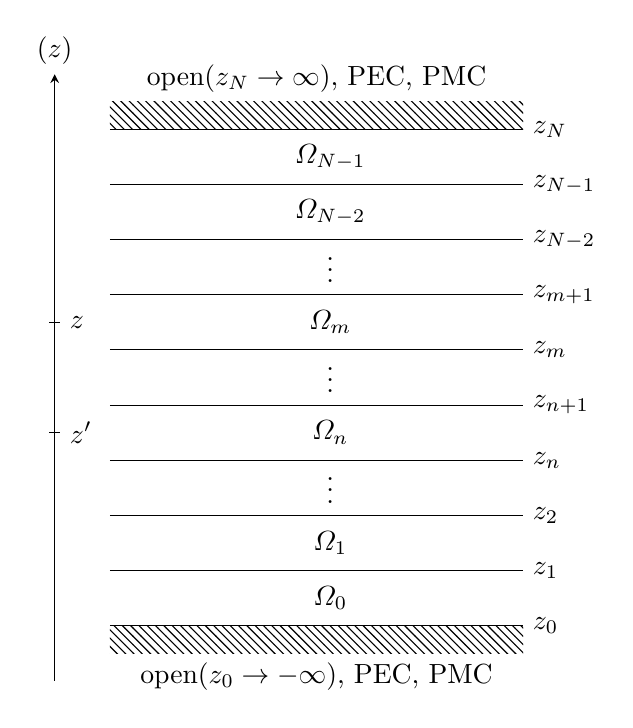
\begin{tikzpicture}[
        scale = 0.7,
		]

        % Coordinate axis
        \draw [->,>=stealth] (-1,-1) -- (-1,10) node[above] {$\left(z\right)$};
        \draw (-1.1,3.5) -- (-0.9,3.5) node[right] {$z^\prime$};
        \draw (-1.1,5.5) -- (-0.9,5.5) node[right] {$z$};

        % Top BC
        \draw[draw=none,pattern=north west lines] (0,9) -- (7.5,9) -- (7.5,9.5)
        --node[above]{open($z_N\to\infty$), PEC, PMC} (0,9.5) -- cycle;

        % Layers
        \draw (0,9) -- (7.5,9) node[right]{$z_{N}$};
        \node at (4,8.5) [align=center] {$\Omega_{N-1}$};
        \draw (0,8) -- (7.5,8) node[right]{$z_{N-1}$};
        \node at (4,7.5) [align=center] {$\Omega_{N-2}$};
        \draw (0,7) -- (7.5,7) node[right]{$z_{N-2}$};
        \node at (4,6.6) [align=center] {\vdots};
        \draw (0,6) -- (7.5,6) node[right]{$z_{m+1}$};
        \node at (4,5.5) [align=center] {$\Omega_m$};
        \draw (0,5) -- (7.5,5) node[right]{$z_m$};
        \node at (4,4.6) [align=center] {\vdots};
        \draw (0,4) -- (7.5,4) node[right]{$z_{n+1}$};
        \node at (4,3.5) [align=center] {$\Omega_n$};
        \draw (0,3) -- (7.5,3) node[right]{$z_n$};
        \node at (4,2.6) [align=center] {\vdots};
        \draw (0,2) -- (7.5,2) node[right]{$z_2$};
        \node at (4,1.5) [align=center] {$\Omega_1$};
        \draw (0,1) -- (7.5,1) node[right]{$z_1$};
        \node at (4,0.5) [align=center] {$\Omega_0$};
        \draw (0,0) --(7.5,0) node[right]{$z_0$};

        % Bottom BC
        \draw[draw=none,pattern=north west lines] (0,0) -- (7.5,0) -- (7.5,-0.5)
        --node[below]{open($z_0\to-\infty$), PEC, PMC} (0,-0.5) -- cycle;
    \end{tikzpicture}
    \caption[Multilayered medium with indexing scheme]
	{Multilayered medium with indexing scheme.
	The layers are defined as domains
	$\Omega_i = \left\{z \in \R\,:\, z_i \leq z < z_{i+1}\right\}$.}
    \label{fig:multilayered_medium_spec}
\end{figure}

According to \cref{fig:multilayered_medium_spec}, discontinuities of $\epsr$ and
$\mur$ may occur at the interface coordinates $z_i$.
Hence, continuity conditions for the characteristic components of \ac{TM} and
\ac{TE} fields need to be derived at these interfaces.
A heuristic way to obtain such conditions is to deduce them directly
from \eqref{eq:TM_characteristic_component_PDE} and
\eqref{eq:TE_characteristic_component_PDE} by requiring existence of all 
involved derivatives \cite[47]{Chew1999}.
Another approach may employ \eqref{eq:mwe_continuity_at_interface}.
Both approaches lead to the continuity conditions
\begin{subequations}\label{eq:TM_continuity}
	\begin{equation}\label{eq:TM_continuity_1}
		\varepsilon_i E_{z} \left(z^{-}\right) =
		\varepsilon_{i-1} E_{z} \left(z^{+}\right)
	\end{equation}
	and
	\begin{equation}\label{eq:TM_continuity_2}
		\frac{1}{\varepsilon_i}
		\frac{\dd}{\dd z}
		\varepsilon_i E_{z}\left(z^{-}\right)
		=
		\frac{1}{\varepsilon_{i+1}}
		\frac{\dd}{\dd z}
		\varepsilon_{i-1} E_{z} \left(z^{+}\right)
		\,,
	\end{equation}
\end{subequations}
for  $\varepsilon E_z$ at a boundary $z_i$, where $z^{\pm} \to z_i$ from both
sides.
Once more the duality principle can be employed to obtain the corresponding
conditions 
\begin{subequations}\label{eq:TE_continuity}
	\begin{equation}\label{eq:TE_continuity_1}
		\mu_i H_{z} \left(z^{-}\right) =
		\mu_{i-1} H_{z} \left(z^{+}\right)
	\end{equation}
	and
	\begin{equation}\label{eq:TE_continuity_2}
		\frac{1}{\mu_i}
		\frac{\dd}{\dd z}
		\mu_i H_{z}\left(z^{-}\right)
		=
		\frac{1}{\mu_{i+1}}
		\frac{\dd}{\dd z}
		\mu_{i-1} H_{z} \left(z^{+}\right)
		\,,
	\end{equation}
\end{subequations}
for $\mu H_z$.








\subsection{Characteristic Field Component for a Vertical Electric Dipole}
\label{subsec:E_z_comp_of_VED}

With \eqref{eq:TM_characteristic_component_PDE} in mind, consider now 
a \ac{VED},~\ie, an infinitesimal $\uv{z}$-directed current element.
As $\varepsilon = \varepsilon\left(z\right)$ and $\mu = \mu\left(z\right)$,
one can, without loss of generality, lay the \ac{VED} onto the Cartesian
and cylindrical $z$-axis with which the current density formally reads
\begin{equation}\label{eq:VED_current_density}
	\pvec{J} \left(\pvec{r}\right) =
	I \uv{z}
	\diracDelta\left(x\right)
	\diracDelta\left(y\right)
	\diracDelta\left(z - z^\prime\right)
	\, .
\end{equation}
As the excitation $\pvec{J}$ has no transverse component, it is a justifiable
assumption that the \ac{VED} field is of azimuthal symmetry.
By the nature of \eqref{eq:mwe_fd_ampere} it can further be deduced that
$\pvec{H}$ has no vertical component.
With these two arguments the \ac{VED} field is known to be \ac{TM} and to depend
on position in the particular way
$\pvec{F} = \pvec{F} \left(\rho, z\right)$,
$\pvec{F} \in \left\{\pvec{E}, \pvec{H}\right\}$.
These characteristics allow for application of the Hankel transform
\eqref{eq:hankel_transform} to \eqref{eq:TM_characteristic_component_PDE}.
Then, with \cref{coll:k_rho_domain}, the \ac{PDE}
\eqref{eq:TM_characteristic_component_PDE} reduces to the \ac{ODE}
\begin{equation}\label{eq:VED_E_z_ODE}
	\left(
		\varepsilon \left(z\right)
		\frac{\dd}{\dd z}
		\frac{1}{\varepsilon \left(z\right)}
		\frac{\dd}{\dd z}
		+
		k_z^2 \left(z\right)
	\right)
	\varepsilon \left(z\right)
	\tilde{E}_z \left(k_\rho, z, z^\prime\right) = 0
	\qquad
	z \neq z^\prime
\end{equation}
in the $k_\rho$ spectral domain, where again the Pythagorean relation
\eqref{eq:def_k_z_of_k_rho} is used for notational convenience.
The Green's function of \eqref{eq:VED_E_z_ODE} defined by
\begin{equation}\label{eq:VED_E_z_ODE_greens_function_def}
	\left(
		\varepsilon \left(z\right)
		\frac{\dd}{\dd z}
		\frac{1}{\varepsilon \left(z\right)}
		\frac{\dd}{\dd z}
		+
		k_z^2 \left(z\right)
	\right)
	\tilde{G}_\mathrm{VED}
	% \tilde{G}^\mathrm{EJ}_{zz} \left(z, z^\prime\right)
	=
	-\diracDelta \left( z - z^\prime \right)
\end{equation}
is then the spectral domain representation of the characteristic component of
the \ac{VED} field.

The spectral-domain solution $\tilde{E}_z$ again obeys Maxwell's equations.
Therefore, spectral domain equations for the remaining field components can be
obtained by differentiation.
The spatial domain solution for each component is then found by inverse Hankel
transformation,~\ie, by means of Sommerfeld integrals.






\subsection{Equivalent Transmission Line Network Method}
\label{subsec:network_method}




\subsubsection{Notion of the Method}

The Green's function of \eqref{eq:VED_E_z_ODE} for the solution domain shown
in \cref{fig:multilayered_medium_spec} can be found by various
procedures \cite{Sommerfeld1964,Chew1999}.
However, from an electrical engineer's perspective it is especially appealing to
not actually \emph{solve} the problem at all but to use familiar results from 
another well-understood area of electrical engineering:
transmission line theory.
It is again the duality principle which makes this possible---and
Feynman's quote (see \cref{sec:duality_principle}) is proved helpful one more
time.
As it turns out, not only the Green's function for \eqref{eq:VED_E_z_ODE} but
actually \emph{all} possible Green's functions arising in the study of
wave propagation in planar multilayered media can be expressed in terms of the
Green's function for voltage and current on an equivalent transmission line
network whose governing \acp{ODE} are dual to those of the field problem in its
$k_\rho$-domain representation \cite{Felsen1994,Michalski2005,Michalski2016b}.

The homogeneous transmission line equations for a $z$-directed line with
wavenumber $k_z$ are given by
\cite{Felsen1994,Michalski2016b}
\begin{subequations}\label{eq:tl_ode_system}
	\begin{align}
		\frac{\dd}{\dd z}
		V^\tx
		+
		\im
		k_z
		Z^\tx
		I^\tx
		&= 0
		\label{eq:tl_ode_system_dV}
		\\
		\frac{\dd}{\dd z}
		I^\tx
		+
		\im
		k_z
		Y^\tx
		V^\tx
		&= 0
		\label{eq:tl_ode_system_dI}
		\, ,
	\end{align}
\end{subequations}
where with regard to the characteristic impedance $Z \equiv Y^{-1}$ a
distinction is made for $\tx \in \left\{\te,\tm\right\}$, \ie, different
characteristic impedances are assumed for transmission lines carrying
\ac{TM} and \ac{TE} modes.
Within the framework of multilayered media the transmission line
characteristics in the $i$-th layer are determined by \cite{Michalski2016b}
\begin{equation}
	k_{zi} = \sqrt{{k_i}^2 - {k_\rho}^2}
	\, ,
\end{equation}
\begin{equation}
	Z_i^\tm = \frac{k_{zi}}{\omega \varepsilon_i}
\end{equation}
and
\begin{equation}
	Z_i^\te = \frac{\omega \mu_i}{k_{zi}}
	\, .
\end{equation}

For the system \eqref{eq:tl_ode_system} Green's functions can be defined in
two ways \cite{Michalski2016b}, namely by excitation with a unit-strength
current source,
\begin{subequations}\label{eq:tl_ode_system_current_gf}
	\begin{align}
		\frac{\dd}{\dd z}
		V_i^\tx
		+
		\im
		k_z
		Z^\tx
		I_i^\tx
		&= 0
		\\
		\frac{\dd}{\dd z}
		I_i^\tx
		+
		\im
		k_z
		Y^\tx
		V_i^\tx
		&= 
		\diracDelta\left(z - z^\prime\right)
		\, ,
	\end{align}
\end{subequations}
and for the voltage driven case
\begin{subequations}\label{eq:tl_ode_system_voltage_gf}
	\begin{align}
		\frac{\dd}{\dd z}
		V_v^\tx
		+
		\im
		k_z
		Z^\tx
		I_v^\tx
		&=
		\diracDelta\left(z - z^\prime\right)
		\\
		\frac{\dd}{\dd z}
		I_v^\tx
		+
		\im
		k_z
		Y^\tx
		V_v^\tx
		&= 
		0
		\, .
	\end{align}
\end{subequations}

From \eqref{eq:tl_ode_system_current_gf} and \eqref{eq:tl_ode_system_voltage_gf}
the two second-order \acp{ODE}
\begin{equation}\label{eq:tl_2nd_order_ode_vsrc}
	\left(
		\frac{\dd}{\dd z}
		\frac{1}{\im k_z Y^\tx}
		\frac{\dd}{\dd z} +
		\frac{k_z^2}{\im k_z Y^\tx}
	\right)
	I_v^\tx
	=
	-\diracDelta \left(z - z^\prime\right)
\end{equation}
and
\begin{equation}\label{eq:tl_2nd_order_ode_isrc}
	\left(
		\frac{\dd}{\dd z}
		\frac{1}{\im k_z Z^\tx}
		\frac{\dd}{\dd z} +
		\frac{k_z^2}{\im k_z Z^\tx}
	\right)
	V_i^\tx
	=
	-\diracDelta \left(z - z^\prime\right)
\end{equation}
can be derived which define the Green's functions for both transmission line
quantities in case of $\diracDelta$-excitation by the respective opposing
source type.
The remaining Green's functions $V_v^\tx$ and $I_i^\tx$ can be obtained via
\eqref{eq:tl_ode_system} once $I_v^\tx$ and $V_i^\tx$ are known.
Noting that \eqref{eq:tl_2nd_order_ode_isrc} and
\eqref{eq:tl_2nd_order_ode_vsrc}
are duals it is even sufficient to only solve either for $I_v^\tx$ or $V_i^\tx$
as the respective other case can be obtained by a simple interchange of
impedance and admittance.
The complete set of substitution rules for the \acp{TLGF} is given by
\cref{tab:tlgf_duality}.

\begin{table}[hbt]
	\centering
	\begin{tabular}{cc}
		\toprule%
		\textbf{original} & \textbf{dual}\\ \midrule
		$V_i$ & $I_v$ \\
		$I_i$ & $V_v$ \\
		$Z$ & $Y$ \\
		\bottomrule
	\end{tabular}
	\caption{Duality substitution rules for \acp{TLGF}.}
	\label{tab:tlgf_duality}
\end{table}

As various literature sources
\cite{Michalski1990,Hsu1993,Ho1994,Eibert1997,Michalski2005}
provide more or less ready to use expressions for the \acp{TLGF}---for special
cases as well as for a general multilayered medium---these results are not
re-considered here in detail.
For the purposes of illustration it is sufficient to give the \acs{TLGF} for
the special case of the classical Sommerfeld problem, \ie, two half-spaces
with open boundary conditions and a single interface at $z = 0$.
In the scheme of \cref{fig:multilayered_medium_spec} the upper (air) half-space
is identified by index $1$.
In this case the fundamental \ac{TLGF} can be chosen to be \cite{Michalski2016b}
\begin{equation}\label{eq:TLGF_V_i}
	V_i^\tx \left(z, z^\prime\right)
	=
	\frac{Z_1^\tx}{2}
	\left(
		\exp{-\im k_1 \abs{z - z^\prime}}
		+
		\overleftarrow{\Gamma}_1^\tx
		\exp{-\im k_1 \left(z - z^\prime\right)}
	\right)
	\, ,
\end{equation}
where
\begin{equation}
	\overleftarrow{\Gamma}_1^\tx
	=
	\frac{Z_0^\tx - Z_1^\tx}{Z_0^\tx + Z_1^\tx}
\end{equation}
is the voltage reflection coefficient looking in negative $z$-direction at the
interface of the two half-spaces.
Note that \eqref{eq:TLGF_V_i} is continuous yet not differentiable in
$z = z^\prime$.
Therefore,
\begin{equation}\label{eq:TLGF_I_I}
	I_i^\tx \left(z, z^\prime\right)
	=
	\frac{1}{2}
	\left(
		\pm
		\exp{-\im k_1 \abs{z - z^\prime}}
		+
		\overleftarrow{\Gamma}_1^\tx
		\exp{-\im k_1 \left(z - z^\prime\right)}
	\right)
	\, ,
\end{equation}
which follows through \eqref{eq:tl_ode_system_dV}, is undefined at the source
coordinate.
With \eqref{eq:TLGF_V_i} and \eqref{eq:TLGF_I_I} known, the \acp{TLGF} for the
voltage-excited case follow by duality.

Note that the first exponential term in \eqref{eq:TLGF_V_i} is just the
numerator of the spectral Green's function of free space as it occurs in the
Sommerfeld identity \eqref{eq:sommerfeld_identity_pos_real_axis}.
As it is now known that all layered media spectral Green's functions can be
expressed in terms of \acp{TLGF}, it is clear that the generalization
as compared to the case of free-space comes from the \emph{reflected}
contributions, \ie, for the half-space case, from the second summand involving
$\overleftarrow{\Gamma}$ in \eqref{eq:TLGF_V_i}.
This means, however, that the \emph{direct term}, \ie, the first exponential
can always be integrated in closed form using \cref{thm:sommerfeld_identity}.

A detail which proves rather useful towards a computer implementation of
\acp{TLGF} that these voltages and currents obey the reciprocity relations
\cite{Michalski2005}
\begin{subequations}\label{eq:tlgf_reciprocity}
	\begin{align}
		V_i
		\left(z , z^\prime\right)
		&=
		V_i
		\left(z^\prime, z\right)
		\\
		I_v
		\left(z, z^\prime\right)
		&=
		I_v
		\left(z^\prime, z\right)
		\\
		V_v
		\left(z , z^\prime\right)
		&=
		-I_i
		\left(z^\prime, z\right)
		\, .
	\end{align}
\end{subequations}

To illustrate the behavior of voltage and current on the equivalent
\ac{TM} transmission line of a Sommerfeld half-space an example is shown in
\cref{fig:tlgf_example}\footnote{Note that the \acp{TLGF} as given by the
simplified expressions \eqref{eq:TLGF_V_i} and \eqref{eq:TLGF_I_I} are not
applicable for $z < 0$. Instead of these simplified forms the computer
implementation with which \cref{fig:tlgf_example} is computed uses a much more
general formulation \cite{Michalski2005}.}.
One clearly observes that the \ac{TLGF} obtained by differentiation, in this
case $I_i$, is discontinuous at $z = z^\prime$ due to the absolute value
in the differentiated function.
The computed impedance $Z = V / I$ is observed to match the characteristic
line impedance for $z > z^\prime$, which is an indicator for the sanity of
the implementation.
A possibly unexpected observation is that the computed impedance is
\emph{negative} in the lower half-space.
This is a consequence of the case distinction for the direct term in
\eqref{eq:TLGF_I_I} between forward and backward traveling waves.
Thus, the impedance for $z < z^\prime$ appears negative but, however,
has the expected absolute value.

\begin{figure}
   \begin{tikzpicture}
    \pgfplotsset{small}
    \matrix {
        \begin{axis}[
            width = \textwidth,
            height = 0.22\textwidth,
            grid = major,
            xlabel = {$z / \lambda_0$},
            ylabel = {$V_i$ in Volt},
            xmin = -2,
            xmax = 4,
        ]
            \addplot [color = blue] table [x = z_by_lambda_0, y = V_re]
			{thesis_tlgf.dat};
            \addplot [color = red] table [x = z_by_lambda_0, y = V_im]
			{thesis_tlgf.dat};
        \end{axis}
        \\
        \begin{axis}[
            width = \textwidth,
            height = 0.22\textwidth,
            grid = major,
            xlabel = {$z / \lambda_0$},
            ylabel = {$I_i$ in Amp\`ere},
            xmin = -2,
            xmax = 4,
        ]
            \addplot [color = blue] table [x = z_by_lambda_0, y = I_re]
			{thesis_tlgf.dat};
            \addplot [color = red] table [x = z_by_lambda_0, y = I_im]
			{thesis_tlgf.dat};
        \end{axis}
        \\
        \begin{axis}[
            width = \textwidth,
            height = 0.22\textwidth,
            grid = major,
            xlabel = {$z / \lambda_0$},
            ylabel = {$Z / Z_0$},
            ytick = {-2, -1, 0, 1},
            xmin = -2,
            xmax = 4,
        ]
            \addplot [color = blue] table [x = z_by_lambda_0, y = Z_rel_re]
			{thesis_tlgf.dat};
            \addplot [color = red] table [x = z_by_lambda_0, y = Z_rel_im]
			{thesis_tlgf.dat};
        \end{axis}
        \\
        };
    \end{tikzpicture}
    \caption{Example case for \acp{TLGF}: the \ac{TM} lines are excited by
	a unit-strength current source at $z^\prime = \lambda_0$, the medium
	is a Sommerfeld non-magnetic half-space with lossy ground specified by
	$\epsr = \num{9.0} - \num{1.0}\im$.}
	\label{fig:tlgf_example}
\end{figure}









\subsubsection{Application to the \acs{VED} Spectral Green's Function}

The equivalent transmission line network method as prescribed above can now be
readily employed in the solution of \eqref{eq:VED_E_z_ODE_greens_function_def}.
Comparison of \eqref{eq:VED_E_z_ODE_greens_function_def} with
\eqref{eq:tl_2nd_order_ode_vsrc}
for the \ac{TM} case reveals the duality of these two equations.
It is thus obtained that
\begin{subequations}\label{eq:VED_E_z_spectral_gf_in_TLGFs}
	\begin{equation}
		\tilde{G}_\mathrm{VED}
		% \tilde{G}^\mathrm{EJ}_{zz} \left(z, z^\prime\right)
		=
		\frac{V_i^\tm}{\im \omega}
	\end{equation}
	as well as
	\begin{equation}
		\frac{1}{\varepsilon}
		\frac{\dd}{\dd z}
		\tilde{G}_\mathrm{VED}
		% \tilde{G}^\mathrm{EJ}_{zz} \left(z, z^\prime\right)
		=
		-
		\frac{V^\tm}{\im \omega}
		\, .
	\end{equation}
\end{subequations}
With \eqref{eq:VED_E_z_spectral_gf_in_TLGFs} the Green's function of
\eqref{eq:VED_E_z_ODE} is represented by the current on an equivalent
transmission line with \ac{TM} characteristics.

It can be shown \cite[pp.~249]{Jin2015} that the field of a \ac{HED} 
possesses both \ac{TM} and \ac{TE} contributions.
Hence, for a \ac{HED} field two characteristic components and, respectively,
two \acp{TLGF} need to be known.
In the transmission line picture this can be interpreted vividly in the way
that the \ac{VED} only excites the \ac{TM} line, while a \ac{HED} excites
both lines simultaneously.








\subsection{Dyadic Green's Functions}
\label{subsec:dyadic_greens_functions}

The problem arising from the combination of solving \eqref{eq:VED_E_z_ODE}
for the excitation specified by \eqref{eq:VED_current_density} defines a Green's
function.
As noted in \cref{subsec:E_z_comp_of_VED}, all five non-vanishing components of
the \ac{VED} field can be derived with knowledge of $\tilde{E}_z$.
This holds for the fields in the spectral domain (by differentiation) as well as
for their counterparts in the spatial domain (Sommerfeld integrals).

The procedure sketched in \cref{subsec:E_z_comp_of_VED} makes particular use of
physical reasoning to derive an \ac{ODE} for the characteristic component of 
the \ac{VED}. 
In contrast to the \ac{VED}, the field of a \ac{HED} has six non-vanishing
components.
It can be shown, however, that the \ac{HED} field can be decomposed into two
five-component fields, one \ac{TM} and one \ac{TE}
\cite{Sommerfeld1926,Sommerfeld1964,Chew1999}
Therefore, in the \ac{HED} case two \acp{ODE} arise describing the two
characteristic components.
The dual cases of \ac{VMD} and \ac{HMD} again follow by duality.

Knowing the fields of \ac{VED} and \ac{HED} is---due to the principles of
duality and linear superposition---sufficient to represent the field of
infinitesimal dipole of arbitrary direction $\uv{l}$ which may be of electric
or magnetic nature.
In practical applications, \eg, numerical solvers, it is, however, more
convenient to assimilate these results into a form which is typically referred
to as dyadic Green's function.
For example the dyadic Green's function of the electric field for electric
excitation $\dyadicGF{EJ}$ yields the electric field of the $\uv{l}$-directed
\ac{HD} via
\begin{equation}
	\pvec{E}_\mathrm{HD} \left(\robs\right) = 
	\iiint\limits_{V}
	\dyadicGF{EJ} \left(\robs, \rsrc\right)
	\cdot
	I \uv{l} \diracDelta \left(\rdiff\right)
	\, 
	\dd \robs 
	\qquad \rsrc \in V
	\, ,
\end{equation}
from which the tensor nature of dyadic Green's functions becomes clear.

In the representation in terms of Cartesian coordinates and basis vectors the
second-rank tensor fields representing dyadic Green's functions can be written
as a superposition
\begin{equation}\label{eq:dyadic_gf_in_cartesian_dyads}
	\dyad{G} = 
	\uv{x}\uv{x} G_{xx} +
	\uv{x}\uv{y} G_{xy} +
	\uv{x}\uv{z} G_{xz} +
	\uv{y}\uv{x} G_{yx} +
	\uv{y}\uv{y} G_{yy} +
	\ldots
	% \uv{y}\uv{z} G_{yz} +
	% \uv{z}\uv{x} G_{zx} +
	% \uv{z}\uv{y} G_{zy} +
	% \uv{z}\uv{z} G_{zz} +
\end{equation}
of dyads.
Alternatively, \eqref{eq:dyadic_gf_in_cartesian_dyads} may be represented
as a $3 \times 3$ matrix in which case the current density vector $\pvec{J}$ is
interpreted as a column vector in the sense of linear algebra.
In the matrix representation the columns of the dyadic Green's functions have
a distinct physical meaning.
For example the $\dyadicGF{EJ} \cdot \uv{x}$ and $\dyadicGF{EJ} \cdot \uv{x}$
represent the electric field of $\uv{x}$ and $\uv{y}$-directed \acp{VED},
respectively, while $\dyadicGF{EJ} \cdot \uv{z}$ is the electric field of
a \ac{VED}.

A comprehensive derivation of all four dyadic Green's functions $\dyadicGF{EJ}$,
$\dyadicGF{EM}$, $\dyadicGF{HJ}$ and $\dyadicGF{HM}$, both in spectral and in
spatial domain is given in the comprehensive encyclopedia contribution by
\textcite{Michalski2005}.
In the Cartesian matrix picture we have the reciprocity relations
\cite{Michalski2005}
\begin{subequations}\label{eq:dgf_reciprocity}
	\begin{align}
	\dyadicGF{EJ}
	\left(\robs, \rsrc\right)
	&= 
	\transpose{\dyadicGF{EJ} \left(\rsrc, \robs\right)}
	\\ 
	\dyadicGF{HM}
	\left(\robs, \rsrc\right)
	&= 
	\transpose{\dyadicGF{HM} \left(\rsrc, \robs\right)}
	\\
	\dyadicGF{EM}
	\left(\robs, \rsrc\right)
	&=
	-\transpose{\dyadicGF{HJ} \left(\rsrc, \robs\right)}
	\end{align}
\end{subequations}
for the dyadic Green's functions, where $\transpose{\mat{A}}$ denotes the
transpose of matrix $\mat{A}$.








\subsection{Generic Scalar Green's Functions}
\label{subsec:generic_scalar_greens_functions}

Dyadic Green's functions as discussed in \cref{subsec:dyadic_greens_functions}
might be the most versatile way to consider electromagnetic Green's functions,
they are certainly not the most elegant way to do so.
Even in the most general case of an arbitrary oblique dipole it can be shown,
that in this worst case scenario only six Sommerfeld integrals have to be
evaluated to obtain the nine components of $\dyadicGF{EJ}$ and $\dyadicGF{HM}$.
For $\dyadicGF{EM}$ and $\dyadicGF{HJ}$ five Sommerfeld integrals are
sufficient.
However, brute-force computation of dyadic Green's functions for $\pvec{E}$
and $\pvec{H}$ in Cartesian matrix representation hardly makes sense in any
theoretical or practical application.
In numerical integral equation methods usually not the Green's functions for
the fields are used.
Instead, potential formulations which possess several advantages are considered
\cite{Michalski1990,Michalski1990a,Michalski1997}.
In analytical considerations it is also common to utilize symmetry properties.
As outlined in \cref{sec:five_component_fields} only three Sommerfeld integrals
are necessary to describe the fields of \ac{VED} and \ac{HED}.
Another example for successful \enquote{scalarization} of the problem is the
original work of Sommerfeld \cite{Sommerfeld1909,Sommerfeld1912} which is almost
entirely built onto scalar considerations.

Nevertheless, there is a certain arbitrariness in the choice which scalar
quantities to choose in order to approach the problem of Green's functions 
in half-space or planar multilayered solution environments.
For example for the \ac{VED} possibilities range from $\varepsilon \tilde{}$
over the transverse component of $\pvec{H}$ to the vector potential $\pvec{A}$
\cite{Michalski2016b}.
Another nowadays somewhat out fashioned quantity which is very similar to the
vector potential is the so-called Hertz potential Sommerfeld himself used.

As the mathematical differences of all of these essentially equivalent
approaches shall not play a role for the purpose of the present thesis another
way to \emph{define} a generic scalar Green's function is employed here.
The notion of this is to simply supplement the Sommerfeld identity given in
\cref{thm:sommerfeld_identity} by a reflected contribution as present in 
\eqref{eq:TLGF_V_i}.
The so defined spectral Green's function shall reduce to
\eqref{eq:sommerfeld_identity_pos_real_axis} in the case of zero reflection, 
\ie, for a single layer of infinite extent or---equivalently---for multiple
layers of equal material parameters.
Furthermore, the generic spectral Green's functions shall be expressed
conveniently by \acp{TLGF}.

In terms of \cref{coll:hankel_transform}, the actual spectral Green's function
of free space in the Sommerfeld identity is clearly identified in
\eqref{eq:sommerfeld_identity_by_inverse_hankel_transform}.
In order to supplement
$\left(\exp{-\im k_z \abs{z - z^\prime}}\right) / \left(2 \im k_z\right)$
by a reflected contribution it makes sense to define generic scalar Green's
functions for the \ac{TM} and \ac{TE} case as
\begin{definition}[Generic scalar Green's functions]
	\label{def:generic_scalar_gf}
	The \emph{generic scalar Green's functions} for the \ac{TM} and \ac{TE}
	reflection case are defined as 
	\begin{equation}\label{eq:def_generic_sgf_tm}
		\genericSgfTM
		\left(z, z^\prime\right)
		\coloneqq	
		\frac{1}{\im \omega \varepsilon_n}
		I_v^\tm
		\left(z, z^\prime\right)
	\end{equation}
	and
	\begin{equation}\label{eq:def_generic_sgf_te}
		\genericSgfTE
		\left(z, z^\prime\right)
		\coloneqq	
		\frac{1}{\im \omega \mu_n}
		V_i^\te
		\left(z, z^\prime\right)
		\, ,
	\end{equation}
	respectively, where $n$ identifies the layer of $z^\prime$.
\end{definition}

The functions of \cref{def:generic_scalar_gf} turn out to be much more 
handy for numerical experimentation than other spectral Green's function,
\eg, single components of dyadic Green's functions.










\chapter{Fast Multipole Method for the Helmholtz Equation}
\label{ch:fmm}

The crucial idea of the \ac{FMM} is to write $\rdiff$ as a sum
\begin{equation}\label{eq:fmm_rdiff_parts}
	\rdiff =
	\left( \robs - \fmmObsGroupCenter              \right) +
	\left( \fmmObsGroupCenter - \fmmSrcGroupCenter \right) -
	\left( \rsrc - \fmmSrcGroupCenter              \right)
\end{equation}
of three vectors, where $\fmmSrcGroupCenter$ and $\fmmObsGroupCenter$ are the
centers of localized groups of source and observation points, respectively.
For notational convenience, the shorthand notations 
$\fmmDiffGroupCenters \coloneqq \fmmObsGroupCenter - \fmmSrcGroupCenter$
and 
$\pvec{d} \coloneqq \left( \robs - \fmmObsGroupCenter \right) - \left( \rsrc - \fmmSrcGroupCenter \right)$
are introduced.
With \eqref{eq:fmm_rdiff_parts}, the Green's function of the Helmholtz equation
can be \emph{factorized} into three terms which represent
\begin{enumerate}
	\item the \emph{aggregation} of a localized source distribution to the
	reference point $\fmmSrcGroupCenter$, 
	\item the \emph{translation} of the combined effect from
	$\fmmSrcGroupCenter$ to the reference point $\fmmObsGroupCenter$ of a
	localized and \enquote{far-away} groups of observation locations
	and finally
	\item the distribution or \emph{disaggregation} of the combined effect from
	$\fmmObsGroupCenter$ to the individual source points.
\end{enumerate}

The conventional \ac{FMM} for the free-space Green's function
of the Helmholtz equation \eqref{eq:scalar_free_space_gf} is based on two
elementary identities which, in the literature \cite{Rokhlin1993,Coifman1993},
are usually assumed to be given or are derived from more general formulas from
handbooks on mathematical functions \cite{Abramowitz2014,Abramowitz2014}.
The aim of this section is to approach these identities from
an electromagnetic perspective to emphasize the underlying idea and to
illustrate why the methods carries the term multipole in its name.

As it is well-known, the Green's function of the Helmholtz equation
\eqref{eq:scalar_helmholtz_equation} is given by
\eqref{eq:scalar_free_space_gf}.
Clearly, $G_0\left(\robs, \rsrc\right)$ is a function of $r$ only for
$\rsrc = 0$ and its expression in spherical coordinates according to
\cref{def:sph_coords} is most trivial.
The expansion of $G_0\left(\robs, \rsrc\right)$ in terms of fundamental
solutions of \eqref{eq:scalar_helmholtz_equation} in spherical coordinates for
the off-centered case $\rsrc \neq 0$ is a classical result in electromagnetic
theory.
For $r > r^\prime$ this so-called \emph{multiple-expansion} is given by
\cite[492]{Jackson2013}
\begin{equation}\label{eq:multipole_expansion_jackson}
	\frac{\exp{-\im k \rdiffNorm}}{4\pi \rdiffNorm} = 
	-\im k \sum_{l = 0}^{\infty}
	\sphbesselj{l} \left(k r^\prime\right)
	\sphbesselh{2}{l} \left(k r\right)
	\sum_{m = -l}^{l}
	\complexConjugate{\operatorname{Y}}_{l m}
	\left( \vartheta^\prime, \varphi^\prime \right) 
	\operatorname{Y}_{l m}
	\left( \vartheta, \varphi\right)
	\qquad
	r > r^\prime
\end{equation}
where $\sphbesselj{l}$ and $\sphbesselh{2}{l}$ are the spherical Bessel and
second-kind spherical Hankel function of $l$-th order, respectively, and
$\operatorname{Y}_{l m}$ denotes the spherical harmonic of $l$-th degree and
$m$-th order.
The variables $\vartheta, \varphi$ and $\vartheta^\prime, \varphi^\prime$ are
the spherical angles of $\robs$ and $\rsrc$, respectively.
The multipole expansion \eqref{eq:multipole_expansion_jackson} is especially
useful if the field of a source distribution of local support within a
\enquote{small} domain is considered for \enquote{far-away} observation points
$\robs$.
For such a configuration the series over $l$ in
\eqref{eq:multipole_expansion_jackson} converges quickly and accurate
approximations can be obtained with relatively few terms.
In the electrostatic version of \eqref{eq:multipole_expansion_jackson},~\ie,
the multipole expansion for the Poisson equation
(obtained form \eqref{eq:scalar_helmholtz_equation} for $k \to 0$) the series
terms correspond to the individual fields of a monopole, dipole, quadrupole,
and so forth, hence this kind of expansion is called multipole expansion.

Towards the form of \eqref{eq:multipole_expansion_jackson} which is used within
the \ac{FMM} it is useful to express the cosine of the angle enclosed by
$\robs$ and $\rsrc$ as
\begin{equation}\label{eq:cos_gamma_sph_coords}
	\uv{r} \cdot \uv{r}^\prime =
	\cos \left(\vartheta\right) \cos \vartheta^\prime +
	\sin \left(\vartheta\right) \sin \left(\vartheta^\prime\right)
	\cos \left(\varphi - \varphi^\prime\right)
	\, .
\end{equation}
With the addition theorem for the spherical harmonics
\cite[(14.30.9)]{Olver2010} and \eqref{eq:cos_gamma_sph_coords} the multipole
series \eqref{eq:multipole_expansion_jackson} can be written
as\footnote{A ground up derivation of \eqref{eq:multiple_expansion_fmm} is
shown in the textbook by \textcite[414]{Stratton2007}}
\begin{equation}\label{eq:multiple_expansion_fmm}
	\frac{\exp{-\im k \rdiffNorm}}{\rdiffNorm} =
	-\im k \sum\limits_{l=0}^{\infty}
	\left(2l + 1\right)
	\sphbesselj{l}    \left( k r^\prime \right)
	\sphbesselh{2}{l} \left( k r        \right)
	\legendrepl{l} \left( \uv{r} \cdot \uv{r^\prime} \right)
	\qquad
	r > r^\prime
	\, .
\end{equation}
The form \eqref{eq:multiple_expansion_fmm} is sometimes called \enquote{addition
theorem for spherical wave functions} \cite[362]{Jin2015} as it expands the
Green's function of the Helmholtz equation in terms of spherical waves for the
off-centered case $\rsrc$.

Now \eqref{eq:multiple_expansion_fmm} is almost the first major \ac{FMM}
identity, as by only flipping the sign of $\rsrc$ we obtain
\begin{lemma}[Gegenbauer's addition theorem]
	Let $\pvec{X}, \pvec{d} \in \R^3$ be two vectors with
	$d < X$ and assume $0 < k \in \R$.
	Then Gegenbauer's addition reads
	\begin{equation}\label{eq:fmm_std_gegenbauer}
		\frac{\exp{-\im k \norm{\pvec{X} + \pvec{d}}}}{\norm{\pvec{X} + \pvec{d}}} = 
		-\im k \sum\limits_{l=0}^{\infty}
		\left( -1 \right)^l
		\left( 2l + 1 \right) \,
		\sphbesselj{l} \left( k d  \right) \,
		\sphbesselh{2}{l} \left( k X \right) \, 
		\legendrepl{l} \left( \uv{X} \cdot  \uv{d} \right)
		\, .
	\end{equation}
\end{lemma} 
\begin{proof}
	By inspection of the respective left-hand sides of
	\eqref{eq:multiple_expansion_fmm} and
	\eqref{eq:fmm_std_gegenbauer} it is observed that $\robs = \pvec{X}$
	and $-\rsrc = \pvec{d}$.
	From the reflection formula of Legendre polynomials
	\cite[(14.7.17)]{Olver2010}
	\begin{equation}\label{eq:legendre_pol_reflection_formula}
		\legendrepl{l} \left( \uv{X} \cdot \uv{d} \right) =
		\legendrepl{l} \left( \uv{r} \cdot \left(-\uv{r}^\prime\right) \right) =
		\legendrepl{l} \left( -\uv{r} \cdot \uv{r}^\prime \right) =
		\left(-1\right)^l \legendrepl{l} \left( \uv{r} \cdot \uv{r}^\prime \right)
	\end{equation}
	it is known that $\legendrepl{l}$ is even (odd) for even (odd) degree $l$.
	As $\uv{X} \cdot \uv{d} = -\uv{r} \cdot \uv{r^\prime} $
	the factor $\left(-1\right)^l$ in \eqref{eq:fmm_std_gegenbauer} follows
	directly from \eqref{eq:legendre_pol_reflection_formula}.
\end{proof}

The second major identity towards \ac{FMM} expands the product 
$\sphbesselj{l} \left( k d \right) \legendrepl{l} \left( \uv{X} \cdot \uv{d} \right)$
in \eqref{eq:fmm_std_gegenbauer} into an integral of weighted propagating plane
waves.
For compact notation, it is useful to introduce
\begin{definition}[Ewald spheren integration]\label{def:ewald_sphere}
	Let $\unitSphereSymbol$ denote the unit sphere in $\R^3$. Then
	integrals of the form
	\begin{equation}\label{eq:ewald_sphere_integral}
		\ewaldintegral f \left(\uv{k}\right) 
		\coloneqq
		\int\limits_{\varphi = 0}^{2\pi} \dd \varphi \, 
		\int\limits_{\vartheta = 0}^{\pi} \dd \vartheta  \, 
		\sin\left(\vartheta \right)
		f \left(\uv{k}\right)
		\, ,
	\end{equation}
	where
	\begin{equation}
		\uv{k} =
		\uv{x} \sin \left(\vartheta\right) \cos \varphi +
		\uv{y} \sin \left(\vartheta\right) \sin \varphi +
		\uv{z} \cos \vartheta \, ,
	\end{equation}
	are said to be an integration over the \emph{Ewald sphere} of propagating
	plane waves.
\end{definition}

\begin{lemma}[Plane wave expansion]
	Let $\pvec{X}, \pvec{d} \in \R^3$ be two vectors with
	$d < X$ and assume $0 < k \in \R$.
	Then we have \cite[410]{Stratton2007}
	\begin{equation}\label{eq:fmm_jP_expansion_plane_waves}
		\sphbesselj{l} \left( k d \right) \,
		\legendrepl{l} \left( \uv{X} \cdot \uv{d} \right) = 
		\frac{\im^l}{4\pi}	
		\ewaldintegral
		\exp{-\im \pvec{k} \cdot \pvec{d}}
		\legendrepl{l} \left( \uv{k} \cdot \uv{X} \right)
		\, .
	\end{equation}
\end{lemma}

Substituting \eqref{eq:fmm_jP_expansion_plane_waves} into
\eqref{eq:fmm_std_gegenbauer} yields
\begin{equation}\label{eq:fmm_before_interchange}
	\frac{\exp{-\im k \norm{\pvec{X} + \pvec{d}}}}{\norm{\pvec{X} + \pvec{d}}} = 
	\frac{-\im k}{4\pi}
	\sum\limits_{l=0}^{\infty}
	\left( -\im \right)^l
	\left( 2l + 1 \right) \,
	\sphbesselh{2}{l} \left( k X \right) 
	\ewaldintegral
	\exp{-\im \pvec{k} \cdot \pvec{d}}
	\legendrepl{l} \left( \uv{k} \cdot \uv{X} \right)
	\, .
\end{equation}
If the multipole expansion is truncated at finite $l$ summation and integration
in \eqref{eq:fmm_before_interchange} can be interchanged
\cite{Rokhlin1993,Coifman1993} to obtain
\begin{equation}\label{eq:fmm_std}
	\frac{\exp{-\im k \norm{\pvec{X} + \pvec{d}}}}{\norm{\pvec{X} + \pvec{d}}}
	\approx 
	\frac{-\im k}{4\pi}
	\ewaldintegral
	\exp{-\im \pvec{k} \cdot \pvec{d}} \,
	\mathcal{T}_L
	\left( \uv{k}, \pvec{X} \right)
	\, ,
\end{equation}
where the quantity
\begin{equation}
	\mathcal{T}_L
	\left( \uv{k}, \pvec{X} \right)
	\coloneqq
	\sum\limits_{l=0}^{L}
	\left( -\im \right)^l
	\left( 2l + 1 \right) \,
	\sphbesselh{2}{l} \left( k X \right) 
	\legendrepl{l} \left( \uv{k} \cdot \uv{X} \right)
	\, ,
\end{equation}
is called \emph{translation operator}.

\chapter{Implementation and Numerical Results}

All results are computed using \texttt{double} precision floating point numbers.

Throughout this chapter relative errors are computed according to
\begin{definition}[Relative error]
    Let $x_\mathrm{r} \neq 0$ be a reference value.
    Then the \emph{relative error} of a result $x_\mathrm{n}$ with respect to
    $x_\mathrm{r}$ is defined by 
    \begin{equation}
        \epsilon \left( x_\mathrm{n} \right) \coloneqq
        20 \log_{10} \abs{\frac{x_\mathrm{n} - x_\mathrm{r}}{x_\mathrm{r}}}
        \SI{}{\decibel}\, .
    \end{equation}
\end{definition}

\section{Numerical Integration of Sommerfeld Integrals}

\cite{Michalski2016a}

Asymptotic behavior \cite{Michalski1998}
\begin{equation}
    \tilde{g}\left(\xi\right)
    \propto \frac{\exp{-\zeta \xi}}{\xi^\alpha}
    \left(C + \mathcal{O}\left(\xi^{-1}\right)\right)
\end{equation}

For Sommerfeld identity: $\xi = \abs{z}$, $\alpha = 1/2$

\begin{figure}
    \centering
    \begin{subfigure}[t]{0.47\textwidth}
    \begin{tikzpicture}
        \begin{axis}[
            width=\textwidth,% subfigure textwidth
            colormap/jet,
            colorbar horizontal,
            colorbar style = {xlabel = {Relative error in $\SI{}{\decibel}$}},
            unbounded coords = jump,
            xlabel = {$\rho / \lambda_0$},
            ylabel = {$z / \lambda_0$},
            xmode = log,
            ymode = log,
            view = {0}{90},
            xtick align=outside,
            ytick align=outside,
            ]
            \addplot3 [
                surf,
                mesh/ordering=y varies,
                ] table[
                    x = x_by_lambda_0, y = z_by_lambda_0, z = rel_err_db,
                ]
                {thesis_numerical_integration_sommerfeld_identity.dat};
        \end{axis}
    \end{tikzpicture}
    \label{fig:production_num_int_sommerfeld_identity:sub1}
    \caption{Relative error. The maximum error is $\SI{-134.42}{\decibel}$.
    At the missing points numerical integration is exact down to machine
    precision.}
    \end{subfigure}
    \hfill
    \begin{subfigure}[t]{0.47\textwidth}
    \begin{tikzpicture}
        \begin{axis}[
            width=\textwidth,% subfigure textwidth
            colormap/jet,
            unbounded coords = jump,
            colorbar horizontal,
            colorbar style = {
                xlabel = {Relative execution time},
                xticklabel = {$10^{\pgfmathprintnumber{\tick}}$},
                },
            xlabel = {$\rho / \lambda_0$},
            ylabel = {$z / \lambda_0$},
            xmode = log,
            ymode = log,
            view = {0}{90},
            xtick align=outside,
            ytick align=outside,
            ]
            \addplot3 [
                surf,
                mesh/ordering=y varies,
                ] table [
                    x = x_by_lambda_0, y = z_by_lambda_0, z expr=log10(\thisrow{rel_time}),
                ]
                {thesis_numerical_integration_sommerfeld_identity.dat};
        \end{axis}
    \end{tikzpicture}
    \label{fig:production_num_int_sommerfeld_identity:sub2}
    \caption{Execution time relative to the point with the fastest execution.
    A total of $\num[]{50}$ evaluations of the Sommerfeld integral are timed
    at each point $\left(\rho,z\right)$.}
    \end{subfigure}

    \caption[Numerical evaluation of the Sommerfeld identity integral]
    {Numerical evaluation of the Sommerfeld identity integral for a source at
    the origin for $10^{-1} \leq a / \lambda_0 \leq 10^{3}$ where
    $a \in \left\{ \rho, z \right\}$.}
\end{figure}

\section{Discrete Complex Image Method}

\section{Fast Multipole Method With Complex Image Sources}


\listoffigures
\listoftables

\printbibliography[heading=bibintoc]

\listoffixmes
    
\end{document}
